% Manuscript. Every number in the text is a macro from generated/numbers.tex, written by
% paper/analysis.py from the saved runs; tables are \input from generated/. Do not type numbers here.
\documentclass[11pt]{article}

\usepackage[a4paper,margin=2.3cm]{geometry}
\usepackage[T1]{fontenc}
\usepackage[utf8]{inputenc}
\usepackage{lmodern}
\usepackage{microtype}
\usepackage{amsmath}
\usepackage{graphicx}
\usepackage{booktabs}
\usepackage{longtable}
\usepackage{array}
\usepackage{xcolor}
\usepackage[font=small,labelfont=bf]{caption}
\usepackage[numbers,sort&compress]{natbib}
\usepackage[colorlinks=true,linkcolor=blue!50!black,citecolor=blue!50!black,urlcolor=blue!50!black]{hyperref}
\usepackage{url}

% Generated by paper/analysis.py - do not edit. One macro per number in the text.
\newcommand{\aucAFiveAaMlp}{0.912}
\newcommand{\aucAFiveBilstm}{0.951}
\newcommand{\aucAFiveBilstmAttn}{0.952}
\newcommand{\aucAFiveCnn}{0.925}
\newcommand{\aucAFiveGbm}{0.950}
\newcommand{\aucAFiveMlp}{0.955}
\newcommand{\aucAFiveTransformer}{0.895}
\newcommand{\aucAFourAaMlp}{0.533}
\newcommand{\aucAFourBilstm}{0.481}
\newcommand{\aucAFourBilstmAttn}{0.608}
\newcommand{\aucAFourCnn}{0.535}
\newcommand{\aucAFourGbm}{0.388}
\newcommand{\aucAFourMlp}{0.414}
\newcommand{\aucAFourTransformer}{0.671}
\newcommand{\aucAOneAaMlp}{0.880}
\newcommand{\aucAOneBilstm}{0.909}
\newcommand{\aucAOneBilstmAttn}{0.918}
\newcommand{\aucAOneCnn}{0.858}
\newcommand{\aucAOneGbm}{0.844}
\newcommand{\aucAOneMlp}{0.918}
\newcommand{\aucAOneTransformer}{0.864}
\newcommand{\aucAThreeAaMlp}{0.778}
\newcommand{\aucAThreeBilstm}{0.766}
\newcommand{\aucAThreeBilstmAttn}{0.781}
\newcommand{\aucAThreeCnn}{0.713}
\newcommand{\aucAThreeGbm}{0.763}
\newcommand{\aucAThreeMlp}{0.810}
\newcommand{\aucAThreeTransformer}{0.773}
\newcommand{\aucATwoAaMlp}{0.802}
\newcommand{\aucATwoBilstm}{0.896}
\newcommand{\aucATwoBilstmAttn}{0.909}
\newcommand{\aucATwoCnn}{0.720}
\newcommand{\aucATwoGbm}{0.875}
\newcommand{\aucATwoMlp}{0.917}
\newcommand{\aucATwoTransformer}{0.756}
\newcommand{\aucAZeroAaMlp}{0.564}
\newcommand{\aucAZeroBilstm}{0.608}
\newcommand{\aucAZeroBilstmAttn}{0.663}
\newcommand{\aucAZeroCnn}{0.512}
\newcommand{\aucAZeroTransformer}{0.713}
\newcommand{\aucBOneAaMlp}{0.907}
\newcommand{\aucBOneBilstm}{0.932}
\newcommand{\aucBOneBilstmAttn}{0.917}
\newcommand{\aucBOneCnn}{0.893}
\newcommand{\aucBOneGbm}{0.939}
\newcommand{\aucBOneMlp}{0.923}
\newcommand{\aucBOneTransformer}{0.897}
\newcommand{\aucBThreeAaMlp}{0.904}
\newcommand{\aucBThreeBilstm}{0.941}
\newcommand{\aucBThreeBilstmAttn}{0.934}
\newcommand{\aucBThreeCnn}{0.889}
\newcommand{\aucBThreeGbm}{0.944}
\newcommand{\aucBThreeMlp}{0.949}
\newcommand{\aucBThreeTransformer}{0.828}
\newcommand{\aucBTwoAaMlp}{0.919}
\newcommand{\aucBTwoBilstm}{0.944}
\newcommand{\aucBTwoBilstmAttn}{0.947}
\newcommand{\aucBTwoCnn}{0.916}
\newcommand{\aucBTwoGbm}{0.925}
\newcommand{\aucBTwoMlp}{0.940}
\newcommand{\aucBTwoTransformer}{0.924}
\newcommand{\aucCiAFiveAaMlp}{[0.884, 0.938]}
\newcommand{\aucCiAFiveBilstm}{[0.928, 0.971]}
\newcommand{\aucCiAFiveBilstmAttn}{[0.930, 0.972]}
\newcommand{\aucCiAFiveCnn}{[0.897, 0.950]}
\newcommand{\aucCiAFiveGbm}{[0.924, 0.972]}
\newcommand{\aucCiAFiveMlp}{[0.930, 0.977]}
\newcommand{\aucCiAFiveTransformer}{[0.863, 0.923]}
\newcommand{\aucCiAFourAaMlp}{[0.481, 0.586]}
\newcommand{\aucCiAFourBilstm}{[0.430, 0.533]}
\newcommand{\aucCiAFourBilstmAttn}{[0.555, 0.661]}
\newcommand{\aucCiAFourCnn}{[0.487, 0.582]}
\newcommand{\aucCiAFourGbm}{[0.326, 0.453]}
\newcommand{\aucCiAFourMlp}{[0.360, 0.470]}
\newcommand{\aucCiAFourTransformer}{[0.620, 0.720]}
\newcommand{\aucCiAOneAaMlp}{[0.843, 0.912]}
\newcommand{\aucCiAOneBilstm}{[0.868, 0.944]}
\newcommand{\aucCiAOneBilstmAttn}{[0.879, 0.951]}
\newcommand{\aucCiAOneCnn}{[0.815, 0.897]}
\newcommand{\aucCiAOneGbm}{[0.798, 0.886]}
\newcommand{\aucCiAOneMlp}{[0.878, 0.953]}
\newcommand{\aucCiAOneTransformer}{[0.823, 0.899]}
\newcommand{\aucCiAThreeAaMlp}{[0.732, 0.821]}
\newcommand{\aucCiAThreeBilstm}{[0.713, 0.814]}
\newcommand{\aucCiAThreeBilstmAttn}{[0.733, 0.825]}
\newcommand{\aucCiAThreeCnn}{[0.662, 0.761]}
\newcommand{\aucCiAThreeGbm}{[0.707, 0.816]}
\newcommand{\aucCiAThreeMlp}{[0.760, 0.855]}
\newcommand{\aucCiAThreeTransformer}{[0.727, 0.815]}
\newcommand{\aucCiATwoAaMlp}{[0.762, 0.839]}
\newcommand{\aucCiATwoBilstm}{[0.863, 0.925]}
\newcommand{\aucCiATwoBilstmAttn}{[0.878, 0.936]}
\newcommand{\aucCiATwoCnn}{[0.676, 0.762]}
\newcommand{\aucCiATwoGbm}{[0.835, 0.910]}
\newcommand{\aucCiATwoMlp}{[0.885, 0.946]}
\newcommand{\aucCiATwoTransformer}{[0.707, 0.800]}
\newcommand{\aucCiAZeroAaMlp}{[0.513, 0.613]}
\newcommand{\aucCiAZeroBilstm}{[0.551, 0.663]}
\newcommand{\aucCiAZeroBilstmAttn}{[0.611, 0.713]}
\newcommand{\aucCiAZeroCnn}{[0.459, 0.564]}
\newcommand{\aucCiAZeroTransformer}{[0.663, 0.761]}
\newcommand{\aucCiBOneAaMlp}{[0.872, 0.937]}
\newcommand{\aucCiBOneBilstm}{[0.896, 0.962]}
\newcommand{\aucCiBOneBilstmAttn}{[0.881, 0.948]}
\newcommand{\aucCiBOneCnn}{[0.847, 0.934]}
\newcommand{\aucCiBOneGbm}{[0.909, 0.965]}
\newcommand{\aucCiBOneMlp}{[0.883, 0.958]}
\newcommand{\aucCiBOneTransformer}{[0.854, 0.934]}
\newcommand{\aucCiBThreeAaMlp}{[0.876, 0.930]}
\newcommand{\aucCiBThreeBilstm}{[0.914, 0.965]}
\newcommand{\aucCiBThreeBilstmAttn}{[0.909, 0.956]}
\newcommand{\aucCiBThreeCnn}{[0.858, 0.917]}
\newcommand{\aucCiBThreeGbm}{[0.915, 0.969]}
\newcommand{\aucCiBThreeMlp}{[0.924, 0.973]}
\newcommand{\aucCiBThreeTransformer}{[0.791, 0.861]}
\newcommand{\aucCiBTwoAaMlp}{[0.893, 0.943]}
\newcommand{\aucCiBTwoBilstm}{[0.922, 0.963]}
\newcommand{\aucCiBTwoBilstmAttn}{[0.926, 0.966]}
\newcommand{\aucCiBTwoCnn}{[0.889, 0.941]}
\newcommand{\aucCiBTwoGbm}{[0.897, 0.950]}
\newcommand{\aucCiBTwoMlp}{[0.914, 0.963]}
\newcommand{\aucCiBTwoTransformer}{[0.899, 0.946]}
\newcommand{\aucCiMAaMlp}{[0.886, 0.938]}
\newcommand{\aucCiMBilstm}{[0.938, 0.982]}
\newcommand{\aucCiMBilstmAttn}{[0.940, 0.984]}
\newcommand{\aucCiMCnn}{[0.881, 0.939]}
\newcommand{\aucCiMGbm}{[0.918, 0.972]}
\newcommand{\aucCiMMlp}{[0.938, 0.982]}
\newcommand{\aucCiMTransformer}{[0.876, 0.938]}
\newcommand{\aucMAaMlp}{0.914}
\newcommand{\aucMBilstm}{0.963}
\newcommand{\aucMBilstmAttn}{0.965}
\newcommand{\aucMCnn}{0.912}
\newcommand{\aucMGbm}{0.948}
\newcommand{\aucMGbmEs}{0.959}
\newcommand{\aucMMlp}{0.962}
\newcommand{\aucMTransformer}{0.910}
\newcommand{\aucObsAFiveGbm}{0.953}
\newcommand{\aucObsAFiveMlp}{0.960}
\newcommand{\aucObsAOneGbm}{0.906}
\newcommand{\aucObsAOneMlp}{0.929}
\newcommand{\aucObsATwoGbm}{0.890}
\newcommand{\aucObsATwoMlp}{0.929}
\newcommand{\aucObsAZeroBilstmAttn}{0.628}
\newcommand{\aucObsBaselineAlphamissense}{0.929}
\newcommand{\aucObsBaselineEsmOneb}{0.911}
\newcommand{\aucObsBaselineNegLogAf}{0.942}
\newcommand{\aucObsCiAFiveGbm}{[0.922, 0.978]}
\newcommand{\aucObsCiAFiveMlp}{[0.928, 0.984]}
\newcommand{\aucObsCiAOneGbm}{[0.862, 0.945]}
\newcommand{\aucObsCiAOneMlp}{[0.887, 0.964]}
\newcommand{\aucObsCiATwoGbm}{[0.841, 0.934]}
\newcommand{\aucObsCiATwoMlp}{[0.887, 0.963]}
\newcommand{\aucObsCiAZeroBilstmAttn}{[0.552, 0.701]}
\newcommand{\aucObsCiBaselineAlphamissense}{[0.887, 0.963]}
\newcommand{\aucObsCiBaselineEsmOneb}{[0.865, 0.951]}
\newcommand{\aucObsCiBaselineNegLogAf}{[0.902, 0.974]}
\newcommand{\aucObsCiMBilstm}{[0.943, 0.988]}
\newcommand{\aucObsCiMGbm}{[0.939, 0.985]}
\newcommand{\aucObsCiMMlp}{[0.932, 0.992]}
\newcommand{\aucObsMBilstm}{0.968}
\newcommand{\aucObsMGbm}{0.965}
\newcommand{\aucObsMMlp}{0.968}
\newcommand{\aucSdAFiveAaMlp}{0.021}
\newcommand{\aucSdAFiveBilstm}{0.009}
\newcommand{\aucSdAFiveBilstmAttn}{0.014}
\newcommand{\aucSdAFiveCnn}{0.005}
\newcommand{\aucSdAFiveGbm}{0.013}
\newcommand{\aucSdAFiveMlp}{0.008}
\newcommand{\aucSdAFiveTransformer}{0.008}
\newcommand{\aucSdAFourAaMlp}{0.018}
\newcommand{\aucSdAFourBilstm}{0.029}
\newcommand{\aucSdAFourBilstmAttn}{0.017}
\newcommand{\aucSdAFourCnn}{0.052}
\newcommand{\aucSdAFourGbm}{0.011}
\newcommand{\aucSdAFourMlp}{0.011}
\newcommand{\aucSdAFourTransformer}{0.013}
\newcommand{\aucSdAOneAaMlp}{0.006}
\newcommand{\aucSdAOneBilstm}{0.002}
\newcommand{\aucSdAOneBilstmAttn}{0.007}
\newcommand{\aucSdAOneCnn}{0.034}
\newcommand{\aucSdAOneGbm}{0.025}
\newcommand{\aucSdAOneMlp}{0.004}
\newcommand{\aucSdAOneTransformer}{0.003}
\newcommand{\aucSdAThreeAaMlp}{0.019}
\newcommand{\aucSdAThreeBilstm}{0.035}
\newcommand{\aucSdAThreeBilstmAttn}{0.009}
\newcommand{\aucSdAThreeCnn}{0.012}
\newcommand{\aucSdAThreeGbm}{0.010}
\newcommand{\aucSdAThreeMlp}{0.026}
\newcommand{\aucSdAThreeTransformer}{0.023}
\newcommand{\aucSdATwoAaMlp}{0.019}
\newcommand{\aucSdATwoBilstm}{0.005}
\newcommand{\aucSdATwoBilstmAttn}{0.008}
\newcommand{\aucSdATwoCnn}{0.020}
\newcommand{\aucSdATwoGbm}{0.003}
\newcommand{\aucSdATwoMlp}{0.000}
\newcommand{\aucSdATwoTransformer}{0.020}
\newcommand{\aucSdAZeroAaMlp}{0.032}
\newcommand{\aucSdAZeroBilstm}{0.038}
\newcommand{\aucSdAZeroBilstmAttn}{0.029}
\newcommand{\aucSdAZeroCnn}{0.044}
\newcommand{\aucSdAZeroTransformer}{0.007}
\newcommand{\aucSdBOneAaMlp}{0.030}
\newcommand{\aucSdBOneBilstm}{0.010}
\newcommand{\aucSdBOneBilstmAttn}{0.030}
\newcommand{\aucSdBOneCnn}{0.005}
\newcommand{\aucSdBOneGbm}{0.003}
\newcommand{\aucSdBOneMlp}{0.010}
\newcommand{\aucSdBOneTransformer}{0.013}
\newcommand{\aucSdBThreeAaMlp}{0.013}
\newcommand{\aucSdBThreeBilstm}{0.007}
\newcommand{\aucSdBThreeBilstmAttn}{0.024}
\newcommand{\aucSdBThreeCnn}{0.026}
\newcommand{\aucSdBThreeGbm}{0.004}
\newcommand{\aucSdBThreeMlp}{0.005}
\newcommand{\aucSdBThreeTransformer}{0.025}
\newcommand{\aucSdBTwoAaMlp}{0.005}
\newcommand{\aucSdBTwoBilstm}{0.006}
\newcommand{\aucSdBTwoBilstmAttn}{0.006}
\newcommand{\aucSdBTwoCnn}{0.014}
\newcommand{\aucSdBTwoGbm}{0.006}
\newcommand{\aucSdBTwoMlp}{0.014}
\newcommand{\aucSdBTwoTransformer}{0.006}
\newcommand{\aucSdMAaMlp}{0.027}
\newcommand{\aucSdMBilstm}{0.001}
\newcommand{\aucSdMBilstmAttn}{0.004}
\newcommand{\aucSdMCnn}{0.006}
\newcommand{\aucSdMGbm}{0.010}
\newcommand{\aucSdMMlp}{0.004}
\newcommand{\aucSdMTransformer}{0.008}
\newcommand{\bOneAucLeast}{$-$0.001}
\newcommand{\bOneAucWorst}{$-$0.038}
\newcommand{\bOneMaxChange}{0.007}
\newcommand{\bTwoMccLeast}{$-$0.116}
\newcommand{\bTwoMccWorst}{$-$0.375}
\newcommand{\baseAlphamissense}{0.917}
\newcommand{\baseCiAlphamissense}{[0.885, 0.946]}
\newcommand{\baseCiEsmOneb}{[0.863, 0.934]}
\newcommand{\baseCiEsmTwo}{[0.855, 0.931]}
\newcommand{\baseCiNegLogAf}{[0.882, 0.956]}
\newcommand{\baseCiRankMean}{[0.950, 0.984]}
\newcommand{\baseEsmOneb}{0.900}
\newcommand{\baseEsmTwo}{0.895}
\newcommand{\baseNegLogAf}{0.922}
\newcommand{\baseRankMean}{0.969}
\newcommand{\benignBsOne}{18}
\newcommand{\benignMLHOne}{31}
\newcommand{\benignMSHSix}{31}
\newcommand{\benignMSHTwo}{56}
\newcommand{\benignObserved}{109}
\newcommand{\benignObservedPct}{89}
\newcommand{\benignPMSTwo}{4}
\newcommand{\benignTotal}{122}
\newcommand{\brierAFiveAaMlp}{0.162}
\newcommand{\brierAFiveBilstm}{0.135}
\newcommand{\brierAFiveBilstmAttn}{0.133}
\newcommand{\brierAFiveCnn}{0.191}
\newcommand{\brierAFiveGbm}{0.071}
\newcommand{\brierAFiveMlp}{0.084}
\newcommand{\brierAFiveTransformer}{0.168}
\newcommand{\brierAFourAaMlp}{0.307}
\newcommand{\brierAFourBilstm}{0.331}
\newcommand{\brierAFourBilstmAttn}{0.349}
\newcommand{\brierAFourCnn}{0.370}
\newcommand{\brierAFourGbm}{0.352}
\newcommand{\brierAFourMlp}{0.299}
\newcommand{\brierAFourTransformer}{0.281}
\newcommand{\brierAOneAaMlp}{0.163}
\newcommand{\brierAOneBilstm}{0.136}
\newcommand{\brierAOneBilstmAttn}{0.129}
\newcommand{\brierAOneCnn}{0.225}
\newcommand{\brierAOneGbm}{0.110}
\newcommand{\brierAOneMlp}{0.126}
\newcommand{\brierAOneTransformer}{0.148}
\newcommand{\brierAThreeAaMlp}{0.204}
\newcommand{\brierAThreeBilstm}{0.205}
\newcommand{\brierAThreeBilstmAttn}{0.212}
\newcommand{\brierAThreeCnn}{0.235}
\newcommand{\brierAThreeGbm}{0.182}
\newcommand{\brierAThreeMlp}{0.182}
\newcommand{\brierAThreeTransformer}{0.208}
\newcommand{\brierATwoAaMlp}{0.206}
\newcommand{\brierATwoBilstm}{0.129}
\newcommand{\brierATwoBilstmAttn}{0.119}
\newcommand{\brierATwoCnn}{0.244}
\newcommand{\brierATwoGbm}{0.121}
\newcommand{\brierATwoMlp}{0.110}
\newcommand{\brierATwoTransformer}{0.231}
\newcommand{\brierAZeroAaMlp}{0.333}
\newcommand{\brierAZeroBilstm}{0.300}
\newcommand{\brierAZeroBilstmAttn}{0.263}
\newcommand{\brierAZeroCnn}{0.374}
\newcommand{\brierAZeroTransformer}{0.262}
\newcommand{\brierBOneAaMlp}{0.231}
\newcommand{\brierBOneBilstm}{0.182}
\newcommand{\brierBOneBilstmAttn}{0.210}
\newcommand{\brierBOneCnn}{0.184}
\newcommand{\brierBOneGbm}{0.360}
\newcommand{\brierBOneMlp}{0.224}
\newcommand{\brierBOneTransformer}{0.239}
\newcommand{\brierBThreeAaMlp}{0.165}
\newcommand{\brierBThreeBilstm}{0.131}
\newcommand{\brierBThreeBilstmAttn}{0.156}
\newcommand{\brierBThreeCnn}{0.209}
\newcommand{\brierBThreeGbm}{0.064}
\newcommand{\brierBThreeMlp}{0.110}
\newcommand{\brierBThreeTransformer}{0.188}
\newcommand{\brierBTwoAaMlp}{0.199}
\newcommand{\brierBTwoBilstm}{0.152}
\newcommand{\brierBTwoBilstmAttn}{0.170}
\newcommand{\brierBTwoCnn}{0.175}
\newcommand{\brierBTwoGbm}{0.255}
\newcommand{\brierBTwoMlp}{0.154}
\newcommand{\brierBTwoTransformer}{0.199}
\newcommand{\brierMAaMlp}{0.166}
\newcommand{\brierMBilstm}{0.093}
\newcommand{\brierMBilstmAttn}{0.089}
\newcommand{\brierMCnn}{0.217}
\newcommand{\brierMGbm}{0.074}
\newcommand{\brierMMlp}{0.076}
\newcommand{\brierMTransformer}{0.132}
\newcommand{\dAucAFiveAaMlpVsAlphamissense}{$-$0.005 [$-$0.038, +0.029]}
\newcommand{\dAucAFiveAaMlpVsAlphamissenseAbs}{0.005}
\newcommand{\dAucAFiveAaMlpVsAlphamissensePoint}{$-$0.005}
\newcommand{\dAucAFiveAaMlpVsNegLogAf}{$-$0.010 [$-$0.041, +0.024]}
\newcommand{\dAucAFiveAaMlpVsNegLogAfAbs}{0.010}
\newcommand{\dAucAFiveAaMlpVsNegLogAfPoint}{$-$0.010}
\newcommand{\dAucAFiveAaMlpVsRankMean}{$-$0.056 [$-$0.080, $-$0.034]}
\newcommand{\dAucAFiveAaMlpVsRankMeanAbs}{0.056}
\newcommand{\dAucAFiveAaMlpVsRankMeanPoint}{$-$0.056}
\newcommand{\dAucAFiveBilstmAttnVsAlphamissense}{+0.035 [+0.005, +0.068]}
\newcommand{\dAucAFiveBilstmAttnVsAlphamissenseAbs}{0.035}
\newcommand{\dAucAFiveBilstmAttnVsAlphamissensePoint}{+0.035}
\newcommand{\dAucAFiveBilstmAttnVsNegLogAf}{+0.031 [+0.002, +0.063]}
\newcommand{\dAucAFiveBilstmAttnVsNegLogAfAbs}{0.031}
\newcommand{\dAucAFiveBilstmAttnVsNegLogAfPoint}{+0.031}
\newcommand{\dAucAFiveBilstmAttnVsRankMean}{$-$0.016 [$-$0.033, $-$0.000]}
\newcommand{\dAucAFiveBilstmAttnVsRankMeanAbs}{0.016}
\newcommand{\dAucAFiveBilstmAttnVsRankMeanPoint}{$-$0.016}
\newcommand{\dAucAFiveBilstmVsAlphamissense}{+0.034 [+0.002, +0.068]}
\newcommand{\dAucAFiveBilstmVsAlphamissenseAbs}{0.034}
\newcommand{\dAucAFiveBilstmVsAlphamissensePoint}{+0.034}
\newcommand{\dAucAFiveBilstmVsNegLogAf}{+0.030 [+0.001, +0.061]}
\newcommand{\dAucAFiveBilstmVsNegLogAfAbs}{0.030}
\newcommand{\dAucAFiveBilstmVsNegLogAfPoint}{+0.030}
\newcommand{\dAucAFiveBilstmVsRankMean}{$-$0.017 [$-$0.034, $-$0.001]}
\newcommand{\dAucAFiveBilstmVsRankMeanAbs}{0.017}
\newcommand{\dAucAFiveBilstmVsRankMeanPoint}{$-$0.017}
\newcommand{\dAucAFiveCnnVsAlphamissense}{+0.008 [$-$0.029, +0.045]}
\newcommand{\dAucAFiveCnnVsAlphamissenseAbs}{0.008}
\newcommand{\dAucAFiveCnnVsAlphamissensePoint}{+0.008}
\newcommand{\dAucAFiveCnnVsNegLogAf}{+0.003 [$-$0.027, +0.036]}
\newcommand{\dAucAFiveCnnVsNegLogAfAbs}{0.003}
\newcommand{\dAucAFiveCnnVsNegLogAfPoint}{+0.003}
\newcommand{\dAucAFiveCnnVsRankMean}{$-$0.044 [$-$0.069, $-$0.021]}
\newcommand{\dAucAFiveCnnVsRankMeanAbs}{0.044}
\newcommand{\dAucAFiveCnnVsRankMeanPoint}{$-$0.044}
\newcommand{\dAucAFiveGbmVsAlphamissense}{+0.032 [+0.004, +0.062]}
\newcommand{\dAucAFiveGbmVsAlphamissenseAbs}{0.032}
\newcommand{\dAucAFiveGbmVsAlphamissensePoint}{+0.032}
\newcommand{\dAucAFiveGbmVsNegLogAf}{+0.028 [$-$0.005, +0.063]}
\newcommand{\dAucAFiveGbmVsNegLogAfAbs}{0.028}
\newcommand{\dAucAFiveGbmVsNegLogAfPoint}{+0.028}
\newcommand{\dAucAFiveGbmVsRankMean}{$-$0.019 [$-$0.037, $-$0.003]}
\newcommand{\dAucAFiveGbmVsRankMeanAbs}{0.019}
\newcommand{\dAucAFiveGbmVsRankMeanPoint}{$-$0.019}
\newcommand{\dAucAFiveMlpVsAlphamissense}{+0.038 [+0.008, +0.069]}
\newcommand{\dAucAFiveMlpVsAlphamissenseAbs}{0.038}
\newcommand{\dAucAFiveMlpVsAlphamissensePoint}{+0.038}
\newcommand{\dAucAFiveMlpVsNegLogAf}{+0.033 [+0.005, +0.065]}
\newcommand{\dAucAFiveMlpVsNegLogAfAbs}{0.033}
\newcommand{\dAucAFiveMlpVsNegLogAfPoint}{+0.033}
\newcommand{\dAucAFiveMlpVsRankMean}{$-$0.014 [$-$0.030, +0.001]}
\newcommand{\dAucAFiveMlpVsRankMeanAbs}{0.014}
\newcommand{\dAucAFiveMlpVsRankMeanPoint}{$-$0.014}
\newcommand{\dAucAFiveTransformerVsAlphamissense}{$-$0.022 [$-$0.061, +0.016]}
\newcommand{\dAucAFiveTransformerVsAlphamissenseAbs}{0.022}
\newcommand{\dAucAFiveTransformerVsAlphamissensePoint}{$-$0.022}
\newcommand{\dAucAFiveTransformerVsNegLogAf}{$-$0.027 [$-$0.062, +0.010]}
\newcommand{\dAucAFiveTransformerVsNegLogAfAbs}{0.027}
\newcommand{\dAucAFiveTransformerVsNegLogAfPoint}{$-$0.027}
\newcommand{\dAucAFiveTransformerVsRankMean}{$-$0.074 [$-$0.102, $-$0.048]}
\newcommand{\dAucAFiveTransformerVsRankMeanAbs}{0.074}
\newcommand{\dAucAFiveTransformerVsRankMeanPoint}{$-$0.074}
\newcommand{\dAucAFiveVsAZeroAaMlp}{+0.348 [+0.297, +0.401]}
\newcommand{\dAucAFiveVsAZeroAaMlpAbs}{0.348}
\newcommand{\dAucAFiveVsAZeroAaMlpPoint}{+0.348}
\newcommand{\dAucAFiveVsAZeroBilstm}{+0.343 [+0.288, +0.401]}
\newcommand{\dAucAFiveVsAZeroBilstmAbs}{0.343}
\newcommand{\dAucAFiveVsAZeroBilstmAttn}{+0.289 [+0.239, +0.342]}
\newcommand{\dAucAFiveVsAZeroBilstmAttnAbs}{0.289}
\newcommand{\dAucAFiveVsAZeroBilstmAttnPoint}{+0.289}
\newcommand{\dAucAFiveVsAZeroBilstmPoint}{+0.343}
\newcommand{\dAucAFiveVsAZeroCnn}{+0.414 [+0.361, +0.467]}
\newcommand{\dAucAFiveVsAZeroCnnAbs}{0.414}
\newcommand{\dAucAFiveVsAZeroCnnPoint}{+0.414}
\newcommand{\dAucAFiveVsAZeroTransformer}{+0.182 [+0.147, +0.219]}
\newcommand{\dAucAFiveVsAZeroTransformerAbs}{0.182}
\newcommand{\dAucAFiveVsAZeroTransformerPoint}{+0.182}
\newcommand{\dAucAFourVsAFiveAaMlp}{$-$0.379 [$-$0.434, $-$0.324]}
\newcommand{\dAucAFourVsAFiveAaMlpAbs}{0.379}
\newcommand{\dAucAFourVsAFiveAaMlpPoint}{$-$0.379}
\newcommand{\dAucAFourVsAFiveBilstm}{$-$0.470 [$-$0.524, $-$0.417]}
\newcommand{\dAucAFourVsAFiveBilstmAbs}{0.470}
\newcommand{\dAucAFourVsAFiveBilstmAttn}{$-$0.344 [$-$0.398, $-$0.291]}
\newcommand{\dAucAFourVsAFiveBilstmAttnAbs}{0.344}
\newcommand{\dAucAFourVsAFiveBilstmAttnPoint}{$-$0.344}
\newcommand{\dAucAFourVsAFiveBilstmPoint}{$-$0.470}
\newcommand{\dAucAFourVsAFiveCnn}{$-$0.390 [$-$0.440, $-$0.342]}
\newcommand{\dAucAFourVsAFiveCnnAbs}{0.390}
\newcommand{\dAucAFourVsAFiveCnnPoint}{$-$0.390}
\newcommand{\dAucAFourVsAFiveGbm}{$-$0.562 [$-$0.625, $-$0.496]}
\newcommand{\dAucAFourVsAFiveGbmAbs}{0.562}
\newcommand{\dAucAFourVsAFiveGbmPoint}{$-$0.562}
\newcommand{\dAucAFourVsAFiveMlp}{$-$0.541 [$-$0.600, $-$0.479]}
\newcommand{\dAucAFourVsAFiveMlpAbs}{0.541}
\newcommand{\dAucAFourVsAFiveMlpPoint}{$-$0.541}
\newcommand{\dAucAFourVsAFiveTransformer}{$-$0.225 [$-$0.268, $-$0.183]}
\newcommand{\dAucAFourVsAFiveTransformerAbs}{0.225}
\newcommand{\dAucAFourVsAFiveTransformerPoint}{$-$0.225}
\newcommand{\dAucAFourVsAZeroAaMlp}{$-$0.031 [$-$0.066, +0.002]}
\newcommand{\dAucAFourVsAZeroAaMlpAbs}{0.031}
\newcommand{\dAucAFourVsAZeroAaMlpPoint}{$-$0.031}
\newcommand{\dAucAFourVsAZeroBilstm}{$-$0.127 [$-$0.182, $-$0.071]}
\newcommand{\dAucAFourVsAZeroBilstmAbs}{0.127}
\newcommand{\dAucAFourVsAZeroBilstmAttn}{$-$0.055 [$-$0.099, $-$0.011]}
\newcommand{\dAucAFourVsAZeroBilstmAttnAbs}{0.055}
\newcommand{\dAucAFourVsAZeroBilstmAttnPoint}{$-$0.055}
\newcommand{\dAucAFourVsAZeroBilstmPoint}{$-$0.127}
\newcommand{\dAucAFourVsAZeroCnn}{+0.024 [$-$0.021, +0.068]}
\newcommand{\dAucAFourVsAZeroCnnAbs}{0.024}
\newcommand{\dAucAFourVsAZeroCnnPoint}{+0.024}
\newcommand{\dAucAFourVsAZeroTransformer}{$-$0.043 [$-$0.076, $-$0.008]}
\newcommand{\dAucAFourVsAZeroTransformerAbs}{0.043}
\newcommand{\dAucAFourVsAZeroTransformerPoint}{$-$0.043}
\newcommand{\dAucAOneVsAFiveAaMlp}{$-$0.033 [$-$0.062, $-$0.005]}
\newcommand{\dAucAOneVsAFiveAaMlpAbs}{0.033}
\newcommand{\dAucAOneVsAFiveAaMlpPoint}{$-$0.033}
\newcommand{\dAucAOneVsAFiveBilstm}{$-$0.043 [$-$0.074, $-$0.015]}
\newcommand{\dAucAOneVsAFiveBilstmAbs}{0.043}
\newcommand{\dAucAOneVsAFiveBilstmAttn}{$-$0.034 [$-$0.065, $-$0.007]}
\newcommand{\dAucAOneVsAFiveBilstmAttnAbs}{0.034}
\newcommand{\dAucAOneVsAFiveBilstmAttnPoint}{$-$0.034}
\newcommand{\dAucAOneVsAFiveBilstmPoint}{$-$0.043}
\newcommand{\dAucAOneVsAFiveCnn}{$-$0.067 [$-$0.099, $-$0.034]}
\newcommand{\dAucAOneVsAFiveCnnAbs}{0.067}
\newcommand{\dAucAOneVsAFiveCnnPoint}{$-$0.067}
\newcommand{\dAucAOneVsAFiveGbm}{$-$0.106 [$-$0.147, $-$0.067]}
\newcommand{\dAucAOneVsAFiveGbmAbs}{0.106}
\newcommand{\dAucAOneVsAFiveGbmPoint}{$-$0.106}
\newcommand{\dAucAOneVsAFiveMlp}{$-$0.036 [$-$0.068, $-$0.009]}
\newcommand{\dAucAOneVsAFiveMlpAbs}{0.036}
\newcommand{\dAucAOneVsAFiveMlpPoint}{$-$0.036}
\newcommand{\dAucAOneVsAFiveTransformer}{$-$0.031 [$-$0.053, $-$0.009]}
\newcommand{\dAucAOneVsAFiveTransformerAbs}{0.031}
\newcommand{\dAucAOneVsAFiveTransformerPoint}{$-$0.031}
\newcommand{\dAucAOneVsAZeroAaMlp}{+0.316 [+0.260, +0.371]}
\newcommand{\dAucAOneVsAZeroAaMlpAbs}{0.316}
\newcommand{\dAucAOneVsAZeroAaMlpPoint}{+0.316}
\newcommand{\dAucAOneVsAZeroBilstm}{+0.301 [+0.243, +0.360]}
\newcommand{\dAucAOneVsAZeroBilstmAbs}{0.301}
\newcommand{\dAucAOneVsAZeroBilstmAttn}{+0.256 [+0.202, +0.309]}
\newcommand{\dAucAOneVsAZeroBilstmAttnAbs}{0.256}
\newcommand{\dAucAOneVsAZeroBilstmAttnPoint}{+0.256}
\newcommand{\dAucAOneVsAZeroBilstmPoint}{+0.301}
\newcommand{\dAucAOneVsAZeroCnn}{+0.347 [+0.292, +0.400]}
\newcommand{\dAucAOneVsAZeroCnnAbs}{0.347}
\newcommand{\dAucAOneVsAZeroCnnPoint}{+0.347}
\newcommand{\dAucAOneVsAZeroTransformer}{+0.151 [+0.118, +0.185]}
\newcommand{\dAucAOneVsAZeroTransformerAbs}{0.151}
\newcommand{\dAucAOneVsAZeroTransformerPoint}{+0.151}
\newcommand{\dAucAThreeVsAFiveAaMlp}{$-$0.135 [$-$0.170, $-$0.101]}
\newcommand{\dAucAThreeVsAFiveAaMlpAbs}{0.135}
\newcommand{\dAucAThreeVsAFiveAaMlpPoint}{$-$0.135}
\newcommand{\dAucAThreeVsAFiveBilstm}{$-$0.185 [$-$0.236, $-$0.138]}
\newcommand{\dAucAThreeVsAFiveBilstmAbs}{0.185}
\newcommand{\dAucAThreeVsAFiveBilstmAttn}{$-$0.171 [$-$0.217, $-$0.127]}
\newcommand{\dAucAThreeVsAFiveBilstmAttnAbs}{0.171}
\newcommand{\dAucAThreeVsAFiveBilstmAttnPoint}{$-$0.171}
\newcommand{\dAucAThreeVsAFiveBilstmPoint}{$-$0.185}
\newcommand{\dAucAThreeVsAFiveCnn}{$-$0.213 [$-$0.254, $-$0.172]}
\newcommand{\dAucAThreeVsAFiveCnnAbs}{0.213}
\newcommand{\dAucAThreeVsAFiveCnnPoint}{$-$0.213}
\newcommand{\dAucAThreeVsAFiveGbm}{$-$0.187 [$-$0.244, $-$0.131]}
\newcommand{\dAucAThreeVsAFiveGbmAbs}{0.187}
\newcommand{\dAucAThreeVsAFiveGbmPoint}{$-$0.187}
\newcommand{\dAucAThreeVsAFiveMlp}{$-$0.145 [$-$0.195, $-$0.098]}
\newcommand{\dAucAThreeVsAFiveMlpAbs}{0.145}
\newcommand{\dAucAThreeVsAFiveMlpPoint}{$-$0.145}
\newcommand{\dAucAThreeVsAFiveTransformer}{$-$0.123 [$-$0.151, $-$0.096]}
\newcommand{\dAucAThreeVsAFiveTransformerAbs}{0.123}
\newcommand{\dAucAThreeVsAFiveTransformerPoint}{$-$0.123}
\newcommand{\dAucAThreeVsAZeroAaMlp}{+0.214 [+0.159, +0.269]}
\newcommand{\dAucAThreeVsAZeroAaMlpAbs}{0.214}
\newcommand{\dAucAThreeVsAZeroAaMlpPoint}{+0.214}
\newcommand{\dAucAThreeVsAZeroBilstm}{+0.158 [+0.101, +0.218]}
\newcommand{\dAucAThreeVsAZeroBilstmAbs}{0.158}
\newcommand{\dAucAThreeVsAZeroBilstmAttn}{+0.118 [+0.065, +0.173]}
\newcommand{\dAucAThreeVsAZeroBilstmAttnAbs}{0.118}
\newcommand{\dAucAThreeVsAZeroBilstmAttnPoint}{+0.118}
\newcommand{\dAucAThreeVsAZeroBilstmPoint}{+0.158}
\newcommand{\dAucAThreeVsAZeroCnn}{+0.201 [+0.147, +0.256]}
\newcommand{\dAucAThreeVsAZeroCnnAbs}{0.201}
\newcommand{\dAucAThreeVsAZeroCnnPoint}{+0.201}
\newcommand{\dAucAThreeVsAZeroTransformer}{+0.059 [+0.033, +0.087]}
\newcommand{\dAucAThreeVsAZeroTransformerAbs}{0.059}
\newcommand{\dAucAThreeVsAZeroTransformerPoint}{+0.059}
\newcommand{\dAucATwoVsAFiveAaMlp}{$-$0.111 [$-$0.147, $-$0.075]}
\newcommand{\dAucATwoVsAFiveAaMlpAbs}{0.111}
\newcommand{\dAucATwoVsAFiveAaMlpPoint}{$-$0.111}
\newcommand{\dAucATwoVsAFiveBilstm}{$-$0.055 [$-$0.090, $-$0.024]}
\newcommand{\dAucATwoVsAFiveBilstmAbs}{0.055}
\newcommand{\dAucATwoVsAFiveBilstmAttn}{$-$0.044 [$-$0.076, $-$0.014]}
\newcommand{\dAucATwoVsAFiveBilstmAttnAbs}{0.044}
\newcommand{\dAucATwoVsAFiveBilstmAttnPoint}{$-$0.044}
\newcommand{\dAucATwoVsAFiveBilstmPoint}{$-$0.055}
\newcommand{\dAucATwoVsAFiveCnn}{$-$0.205 [$-$0.250, $-$0.161]}
\newcommand{\dAucATwoVsAFiveCnnAbs}{0.205}
\newcommand{\dAucATwoVsAFiveCnnPoint}{$-$0.205}
\newcommand{\dAucATwoVsAFiveGbm}{$-$0.074 [$-$0.110, $-$0.042]}
\newcommand{\dAucATwoVsAFiveGbmAbs}{0.074}
\newcommand{\dAucATwoVsAFiveGbmPoint}{$-$0.074}
\newcommand{\dAucATwoVsAFiveMlp}{$-$0.038 [$-$0.069, $-$0.008]}
\newcommand{\dAucATwoVsAFiveMlpAbs}{0.038}
\newcommand{\dAucATwoVsAFiveMlpPoint}{$-$0.038}
\newcommand{\dAucATwoVsAFiveTransformer}{$-$0.139 [$-$0.173, $-$0.107]}
\newcommand{\dAucATwoVsAFiveTransformerAbs}{0.139}
\newcommand{\dAucATwoVsAFiveTransformerPoint}{$-$0.139}
\newcommand{\dAucATwoVsAZeroAaMlp}{+0.238 [+0.193, +0.284]}
\newcommand{\dAucATwoVsAZeroAaMlpAbs}{0.238}
\newcommand{\dAucATwoVsAZeroAaMlpPoint}{+0.238}
\newcommand{\dAucATwoVsAZeroBilstm}{+0.288 [+0.232, +0.346]}
\newcommand{\dAucATwoVsAZeroBilstmAbs}{0.288}
\newcommand{\dAucATwoVsAZeroBilstmAttn}{+0.246 [+0.193, +0.299]}
\newcommand{\dAucATwoVsAZeroBilstmAttnAbs}{0.246}
\newcommand{\dAucATwoVsAZeroBilstmAttnPoint}{+0.246}
\newcommand{\dAucATwoVsAZeroBilstmPoint}{+0.288}
\newcommand{\dAucATwoVsAZeroCnn}{+0.208 [+0.160, +0.257]}
\newcommand{\dAucATwoVsAZeroCnnAbs}{0.208}
\newcommand{\dAucATwoVsAZeroCnnPoint}{+0.208}
\newcommand{\dAucATwoVsAZeroTransformer}{+0.043 [+0.022, +0.064]}
\newcommand{\dAucATwoVsAZeroTransformerAbs}{0.043}
\newcommand{\dAucATwoVsAZeroTransformerPoint}{+0.043}
\newcommand{\dAucAaMlpVsGbmAFive}{$-$0.037 [$-$0.063, $-$0.011]}
\newcommand{\dAucAaMlpVsGbmAFiveAbs}{0.037}
\newcommand{\dAucAaMlpVsGbmAFivePoint}{$-$0.037}
\newcommand{\dAucAaMlpVsGbmM}{$-$0.034 [$-$0.058, $-$0.010]}
\newcommand{\dAucAaMlpVsGbmMAbs}{0.034}
\newcommand{\dAucAaMlpVsGbmMPoint}{$-$0.034}
\newcommand{\dAucBOneVsAFiveAaMlp}{$-$0.012 [$-$0.044, +0.020]}
\newcommand{\dAucBOneVsAFiveAaMlpAbs}{0.012}
\newcommand{\dAucBOneVsAFiveAaMlpPoint}{$-$0.012}
\newcommand{\dAucBOneVsAFiveBilstm}{$-$0.026 [$-$0.063, +0.009]}
\newcommand{\dAucBOneVsAFiveBilstmAbs}{0.026}
\newcommand{\dAucBOneVsAFiveBilstmAttn}{$-$0.034 [$-$0.071, +0.001]}
\newcommand{\dAucBOneVsAFiveBilstmAttnAbs}{0.034}
\newcommand{\dAucBOneVsAFiveBilstmAttnPoint}{$-$0.034}
\newcommand{\dAucBOneVsAFiveBilstmPoint}{$-$0.026}
\newcommand{\dAucBOneVsAFiveCnn}{$-$0.038 [$-$0.091, +0.014]}
\newcommand{\dAucBOneVsAFiveCnnAbs}{0.038}
\newcommand{\dAucBOneVsAFiveCnnPoint}{$-$0.038}
\newcommand{\dAucBOneVsAFiveGbm}{$-$0.036 [$-$0.066, $-$0.008]}
\newcommand{\dAucBOneVsAFiveGbmAbs}{0.036}
\newcommand{\dAucBOneVsAFiveGbmPoint}{$-$0.036}
\newcommand{\dAucBOneVsAFiveMlp}{$-$0.037 [$-$0.074, $-$0.003]}
\newcommand{\dAucBOneVsAFiveMlpAbs}{0.037}
\newcommand{\dAucBOneVsAFiveMlpPoint}{$-$0.037}
\newcommand{\dAucBOneVsAFiveTransformer}{$-$0.001 [$-$0.052, +0.052]}
\newcommand{\dAucBOneVsAFiveTransformerAbs}{0.001}
\newcommand{\dAucBOneVsAFiveTransformerPoint}{$-$0.001}
\newcommand{\dAucBThreeVsAFiveAaMlp}{$-$0.008 [$-$0.021, +0.005]}
\newcommand{\dAucBThreeVsAFiveAaMlpAbs}{0.008}
\newcommand{\dAucBThreeVsAFiveAaMlpPoint}{$-$0.008}
\newcommand{\dAucBThreeVsAFiveBilstm}{$-$0.011 [$-$0.031, +0.005]}
\newcommand{\dAucBThreeVsAFiveBilstmAbs}{0.011}
\newcommand{\dAucBThreeVsAFiveBilstmAttn}{$-$0.019 [$-$0.032, $-$0.007]}
\newcommand{\dAucBThreeVsAFiveBilstmAttnAbs}{0.019}
\newcommand{\dAucBThreeVsAFiveBilstmAttnPoint}{$-$0.019}
\newcommand{\dAucBThreeVsAFiveBilstmPoint}{$-$0.011}
\newcommand{\dAucBThreeVsAFiveCnn}{$-$0.036 [$-$0.054, $-$0.021]}
\newcommand{\dAucBThreeVsAFiveCnnAbs}{0.036}
\newcommand{\dAucBThreeVsAFiveCnnPoint}{$-$0.036}
\newcommand{\dAucBThreeVsAFiveGbm}{$-$0.006 [$-$0.018, +0.005]}
\newcommand{\dAucBThreeVsAFiveGbmAbs}{0.006}
\newcommand{\dAucBThreeVsAFiveGbmPoint}{$-$0.006}
\newcommand{\dAucBThreeVsAFiveMlp}{$-$0.006 [$-$0.016, +0.003]}
\newcommand{\dAucBThreeVsAFiveMlpAbs}{0.006}
\newcommand{\dAucBThreeVsAFiveMlpPoint}{$-$0.006}
\newcommand{\dAucBThreeVsAFiveTransformer}{$-$0.068 [$-$0.095, $-$0.042]}
\newcommand{\dAucBThreeVsAFiveTransformerAbs}{0.068}
\newcommand{\dAucBThreeVsAFiveTransformerPoint}{$-$0.068}
\newcommand{\dAucBTwoVsAFiveAaMlp}{+0.010 [$-$0.023, +0.044]}
\newcommand{\dAucBTwoVsAFiveAaMlpAbs}{0.010}
\newcommand{\dAucBTwoVsAFiveAaMlpPoint}{+0.010}
\newcommand{\dAucBTwoVsAFiveBilstm}{$-$0.011 [$-$0.041, +0.019]}
\newcommand{\dAucBTwoVsAFiveBilstmAbs}{0.011}
\newcommand{\dAucBTwoVsAFiveBilstmAttn}{$-$0.008 [$-$0.036, +0.022]}
\newcommand{\dAucBTwoVsAFiveBilstmAttnAbs}{0.008}
\newcommand{\dAucBTwoVsAFiveBilstmAttnPoint}{$-$0.008}
\newcommand{\dAucBTwoVsAFiveBilstmPoint}{$-$0.011}
\newcommand{\dAucBTwoVsAFiveCnn}{$-$0.013 [$-$0.056, +0.032]}
\newcommand{\dAucBTwoVsAFiveCnnAbs}{0.013}
\newcommand{\dAucBTwoVsAFiveCnnPoint}{$-$0.013}
\newcommand{\dAucBTwoVsAFiveGbm}{$-$0.037 [$-$0.067, $-$0.006]}
\newcommand{\dAucBTwoVsAFiveGbmAbs}{0.037}
\newcommand{\dAucBTwoVsAFiveGbmPoint}{$-$0.037}
\newcommand{\dAucBTwoVsAFiveMlp}{$-$0.022 [$-$0.050, +0.006]}
\newcommand{\dAucBTwoVsAFiveMlpAbs}{0.022}
\newcommand{\dAucBTwoVsAFiveMlpPoint}{$-$0.022}
\newcommand{\dAucBTwoVsAFiveTransformer}{+0.043 [+0.004, +0.084]}
\newcommand{\dAucBTwoVsAFiveTransformerAbs}{0.043}
\newcommand{\dAucBTwoVsAFiveTransformerPoint}{+0.043}
\newcommand{\dAucBilstmAttnVsGbmAFive}{+0.003 [$-$0.016, +0.022]}
\newcommand{\dAucBilstmAttnVsGbmAFiveAbs}{0.003}
\newcommand{\dAucBilstmAttnVsGbmAFivePoint}{+0.003}
\newcommand{\dAucBilstmAttnVsGbmM}{+0.017 [$-$0.001, +0.036]}
\newcommand{\dAucBilstmAttnVsGbmMAbs}{0.017}
\newcommand{\dAucBilstmAttnVsGbmMPoint}{+0.017}
\newcommand{\dAucBilstmVsGbmAFive}{+0.002 [$-$0.018, +0.021]}
\newcommand{\dAucBilstmVsGbmAFiveAbs}{0.002}
\newcommand{\dAucBilstmVsGbmAFivePoint}{+0.002}
\newcommand{\dAucBilstmVsGbmM}{+0.015 [$-$0.004, +0.035]}
\newcommand{\dAucBilstmVsGbmMAbs}{0.015}
\newcommand{\dAucBilstmVsGbmMPoint}{+0.015}
\newcommand{\dAucCnnVsGbmAFive}{$-$0.024 [$-$0.051, +0.002]}
\newcommand{\dAucCnnVsGbmAFiveAbs}{0.024}
\newcommand{\dAucCnnVsGbmAFivePoint}{$-$0.024}
\newcommand{\dAucCnnVsGbmM}{$-$0.036 [$-$0.064, $-$0.010]}
\newcommand{\dAucCnnVsGbmMAbs}{0.036}
\newcommand{\dAucCnnVsGbmMPoint}{$-$0.036}
\newcommand{\dAucGbmEsVsGbm}{+0.011 [+0.004, +0.020]}
\newcommand{\dAucGbmEsVsMlp}{$-$0.003 [$-$0.014, +0.009]}
\newcommand{\dAucMAaMlpVsAlphamissense}{$-$0.004 [$-$0.037, +0.032]}
\newcommand{\dAucMAaMlpVsAlphamissenseAbs}{0.004}
\newcommand{\dAucMAaMlpVsAlphamissensePoint}{$-$0.004}
\newcommand{\dAucMAaMlpVsNegLogAf}{$-$0.008 [$-$0.038, +0.025]}
\newcommand{\dAucMAaMlpVsNegLogAfAbs}{0.008}
\newcommand{\dAucMAaMlpVsNegLogAfPoint}{$-$0.008}
\newcommand{\dAucMAaMlpVsRankMean}{$-$0.055 [$-$0.075, $-$0.036]}
\newcommand{\dAucMAaMlpVsRankMeanAbs}{0.055}
\newcommand{\dAucMAaMlpVsRankMeanPoint}{$-$0.055}
\newcommand{\dAucMBilstmAttnVsAlphamissense}{+0.047 [+0.016, +0.080]}
\newcommand{\dAucMBilstmAttnVsAlphamissenseAbs}{0.047}
\newcommand{\dAucMBilstmAttnVsAlphamissensePoint}{+0.047}
\newcommand{\dAucMBilstmAttnVsNegLogAf}{+0.043 [+0.018, +0.073]}
\newcommand{\dAucMBilstmAttnVsNegLogAfAbs}{0.043}
\newcommand{\dAucMBilstmAttnVsNegLogAfPoint}{+0.043}
\newcommand{\dAucMBilstmAttnVsRankMean}{$-$0.004 [$-$0.017, +0.008]}
\newcommand{\dAucMBilstmAttnVsRankMeanAbs}{0.004}
\newcommand{\dAucMBilstmAttnVsRankMeanPoint}{$-$0.004}
\newcommand{\dAucMBilstmVsAlphamissense}{+0.045 [+0.014, +0.078]}
\newcommand{\dAucMBilstmVsAlphamissenseAbs}{0.045}
\newcommand{\dAucMBilstmVsAlphamissensePoint}{+0.045}
\newcommand{\dAucMBilstmVsNegLogAf}{+0.041 [+0.018, +0.068]}
\newcommand{\dAucMBilstmVsNegLogAfAbs}{0.041}
\newcommand{\dAucMBilstmVsNegLogAfPoint}{+0.041}
\newcommand{\dAucMBilstmVsRankMean}{$-$0.006 [$-$0.019, +0.006]}
\newcommand{\dAucMBilstmVsRankMeanAbs}{0.006}
\newcommand{\dAucMBilstmVsRankMeanPoint}{$-$0.006}
\newcommand{\dAucMCnnVsAlphamissense}{$-$0.006 [$-$0.043, +0.031]}
\newcommand{\dAucMCnnVsAlphamissenseAbs}{0.006}
\newcommand{\dAucMCnnVsAlphamissensePoint}{$-$0.006}
\newcommand{\dAucMCnnVsNegLogAf}{$-$0.010 [$-$0.039, +0.019]}
\newcommand{\dAucMCnnVsNegLogAfAbs}{0.010}
\newcommand{\dAucMCnnVsNegLogAfPoint}{$-$0.010}
\newcommand{\dAucMCnnVsRankMean}{$-$0.057 [$-$0.081, $-$0.036]}
\newcommand{\dAucMCnnVsRankMeanAbs}{0.057}
\newcommand{\dAucMCnnVsRankMeanPoint}{$-$0.057}
\newcommand{\dAucMGbmVsAlphamissense}{+0.031 [$-$0.001, +0.062]}
\newcommand{\dAucMGbmVsAlphamissenseAbs}{0.031}
\newcommand{\dAucMGbmVsAlphamissensePoint}{+0.031}
\newcommand{\dAucMGbmVsNegLogAf}{+0.026 [$-$0.006, +0.060]}
\newcommand{\dAucMGbmVsNegLogAfAbs}{0.026}
\newcommand{\dAucMGbmVsNegLogAfPoint}{+0.026}
\newcommand{\dAucMGbmVsRankMean}{$-$0.021 [$-$0.040, $-$0.005]}
\newcommand{\dAucMGbmVsRankMeanAbs}{0.021}
\newcommand{\dAucMGbmVsRankMeanPoint}{$-$0.021}
\newcommand{\dAucMMlpVsAlphamissense}{+0.045 [+0.015, +0.076]}
\newcommand{\dAucMMlpVsAlphamissenseAbs}{0.045}
\newcommand{\dAucMMlpVsAlphamissensePoint}{+0.045}
\newcommand{\dAucMMlpVsNegLogAf}{+0.040 [+0.013, +0.071]}
\newcommand{\dAucMMlpVsNegLogAfAbs}{0.040}
\newcommand{\dAucMMlpVsNegLogAfPoint}{+0.040}
\newcommand{\dAucMMlpVsRankMean}{$-$0.006 [$-$0.021, +0.005]}
\newcommand{\dAucMMlpVsRankMeanAbs}{0.006}
\newcommand{\dAucMMlpVsRankMeanPoint}{$-$0.006}
\newcommand{\dAucMTransformerVsAlphamissense}{$-$0.007 [$-$0.047, +0.032]}
\newcommand{\dAucMTransformerVsAlphamissenseAbs}{0.007}
\newcommand{\dAucMTransformerVsAlphamissensePoint}{$-$0.007}
\newcommand{\dAucMTransformerVsNegLogAf}{$-$0.012 [$-$0.044, +0.023]}
\newcommand{\dAucMTransformerVsNegLogAfAbs}{0.012}
\newcommand{\dAucMTransformerVsNegLogAfPoint}{$-$0.012}
\newcommand{\dAucMTransformerVsRankMean}{$-$0.059 [$-$0.086, $-$0.034]}
\newcommand{\dAucMTransformerVsRankMeanAbs}{0.059}
\newcommand{\dAucMTransformerVsRankMeanPoint}{$-$0.059}
\newcommand{\dAucMVsAFiveAaMlp}{+0.001 [$-$0.019, +0.022]}
\newcommand{\dAucMVsAFiveAaMlpAbs}{0.001}
\newcommand{\dAucMVsAFiveAaMlpPoint}{+0.001}
\newcommand{\dAucMVsAFiveBilstm}{+0.011 [$-$0.004, +0.025]}
\newcommand{\dAucMVsAFiveBilstmAbs}{0.011}
\newcommand{\dAucMVsAFiveBilstmAttn}{+0.012 [$-$0.005, +0.028]}
\newcommand{\dAucMVsAFiveBilstmAttnAbs}{0.012}
\newcommand{\dAucMVsAFiveBilstmAttnPoint}{+0.012}
\newcommand{\dAucMVsAFiveBilstmPoint}{+0.011}
\newcommand{\dAucMVsAFiveCnn}{$-$0.014 [$-$0.039, +0.012]}
\newcommand{\dAucMVsAFiveCnnAbs}{0.014}
\newcommand{\dAucMVsAFiveCnnPoint}{$-$0.014}
\newcommand{\dAucMVsAFiveGbm}{$-$0.002 [$-$0.015, +0.011]}
\newcommand{\dAucMVsAFiveGbmAbs}{0.002}
\newcommand{\dAucMVsAFiveGbmPoint}{$-$0.002}
\newcommand{\dAucMVsAFiveMlp}{+0.007 [$-$0.002, +0.017]}
\newcommand{\dAucMVsAFiveMlpAbs}{0.007}
\newcommand{\dAucMVsAFiveMlpPoint}{+0.007}
\newcommand{\dAucMVsAFiveTransformer}{+0.015 [$-$0.003, +0.033]}
\newcommand{\dAucMVsAFiveTransformerAbs}{0.015}
\newcommand{\dAucMVsAFiveTransformerPoint}{+0.015}
\newcommand{\dAucMlpVsGbmAFive}{+0.005 [$-$0.011, +0.021]}
\newcommand{\dAucMlpVsGbmAFiveAbs}{0.005}
\newcommand{\dAucMlpVsGbmAFivePoint}{+0.005}
\newcommand{\dAucMlpVsGbmM}{+0.014 [$-$0.001, +0.031]}
\newcommand{\dAucMlpVsGbmMAbs}{0.014}
\newcommand{\dAucMlpVsGbmMPoint}{+0.014}
\newcommand{\dAucTransformerVsGbmAFive}{$-$0.054 [$-$0.087, $-$0.023]}
\newcommand{\dAucTransformerVsGbmAFiveAbs}{0.054}
\newcommand{\dAucTransformerVsGbmAFivePoint}{$-$0.054}
\newcommand{\dAucTransformerVsGbmM}{$-$0.038 [$-$0.072, $-$0.002]}
\newcommand{\dAucTransformerVsGbmMAbs}{0.038}
\newcommand{\dAucTransformerVsGbmMPoint}{$-$0.038}
\newcommand{\dMccAFiveVsAZeroAaMlp}{+0.455 [+0.370, +0.537]}
\newcommand{\dMccAFiveVsAZeroAaMlpAbs}{0.455}
\newcommand{\dMccAFiveVsAZeroAaMlpPoint}{+0.455}
\newcommand{\dMccAFiveVsAZeroBilstm}{+0.478 [+0.394, +0.560]}
\newcommand{\dMccAFiveVsAZeroBilstmAbs}{0.478}
\newcommand{\dMccAFiveVsAZeroBilstmAttn}{+0.434 [+0.351, +0.516]}
\newcommand{\dMccAFiveVsAZeroBilstmAttnAbs}{0.434}
\newcommand{\dMccAFiveVsAZeroBilstmAttnPoint}{+0.434}
\newcommand{\dMccAFiveVsAZeroBilstmPoint}{+0.478}
\newcommand{\dMccAFiveVsAZeroCnn}{+0.527 [+0.449, +0.600]}
\newcommand{\dMccAFiveVsAZeroCnnAbs}{0.527}
\newcommand{\dMccAFiveVsAZeroCnnPoint}{+0.527}
\newcommand{\dMccAFiveVsAZeroTransformer}{+0.285 [+0.211, +0.357]}
\newcommand{\dMccAFiveVsAZeroTransformerAbs}{0.285}
\newcommand{\dMccAFiveVsAZeroTransformerPoint}{+0.285}
\newcommand{\dMccAFourVsAFiveAaMlp}{$-$0.540 [$-$0.619, $-$0.448]}
\newcommand{\dMccAFourVsAFiveAaMlpAbs}{0.540}
\newcommand{\dMccAFourVsAFiveAaMlpPoint}{$-$0.540}
\newcommand{\dMccAFourVsAFiveBilstm}{$-$0.506 [$-$0.578, $-$0.437]}
\newcommand{\dMccAFourVsAFiveBilstmAbs}{0.506}
\newcommand{\dMccAFourVsAFiveBilstmAttn}{$-$0.465 [$-$0.552, $-$0.378]}
\newcommand{\dMccAFourVsAFiveBilstmAttnAbs}{0.465}
\newcommand{\dMccAFourVsAFiveBilstmAttnPoint}{$-$0.465}
\newcommand{\dMccAFourVsAFiveBilstmPoint}{$-$0.506}
\newcommand{\dMccAFourVsAFiveCnn}{$-$0.526 [$-$0.608, $-$0.444]}
\newcommand{\dMccAFourVsAFiveCnnAbs}{0.526}
\newcommand{\dMccAFourVsAFiveCnnPoint}{$-$0.526}
\newcommand{\dMccAFourVsAFiveGbm}{$-$0.837 [$-$0.934, $-$0.738]}
\newcommand{\dMccAFourVsAFiveGbmAbs}{0.837}
\newcommand{\dMccAFourVsAFiveGbmPoint}{$-$0.837}
\newcommand{\dMccAFourVsAFiveMlp}{$-$0.719 [$-$0.795, $-$0.640]}
\newcommand{\dMccAFourVsAFiveMlpAbs}{0.719}
\newcommand{\dMccAFourVsAFiveMlpPoint}{$-$0.719}
\newcommand{\dMccAFourVsAFiveTransformer}{$-$0.316 [$-$0.391, $-$0.240]}
\newcommand{\dMccAFourVsAFiveTransformerAbs}{0.316}
\newcommand{\dMccAFourVsAFiveTransformerPoint}{$-$0.316}
\newcommand{\dMccAFourVsAZeroAaMlp}{$-$0.085 [$-$0.143, $-$0.020]}
\newcommand{\dMccAFourVsAZeroAaMlpAbs}{0.085}
\newcommand{\dMccAFourVsAZeroAaMlpPoint}{$-$0.085}
\newcommand{\dMccAFourVsAZeroBilstm}{$-$0.028 [$-$0.106, +0.049]}
\newcommand{\dMccAFourVsAZeroBilstmAbs}{0.028}
\newcommand{\dMccAFourVsAZeroBilstmAttn}{$-$0.031 [$-$0.116, +0.054]}
\newcommand{\dMccAFourVsAZeroBilstmAttnAbs}{0.031}
\newcommand{\dMccAFourVsAZeroBilstmAttnPoint}{$-$0.031}
\newcommand{\dMccAFourVsAZeroBilstmPoint}{$-$0.028}
\newcommand{\dMccAFourVsAZeroCnn}{+0.001 [$-$0.075, +0.077]}
\newcommand{\dMccAFourVsAZeroCnnAbs}{0.001}
\newcommand{\dMccAFourVsAZeroCnnPoint}{+0.001}
\newcommand{\dMccAFourVsAZeroTransformer}{$-$0.031 [$-$0.100, +0.041]}
\newcommand{\dMccAFourVsAZeroTransformerAbs}{0.031}
\newcommand{\dMccAFourVsAZeroTransformerPoint}{$-$0.031}
\newcommand{\dMccAOneVsAFiveAaMlp}{$-$0.020 [$-$0.085, +0.046]}
\newcommand{\dMccAOneVsAFiveAaMlpAbs}{0.020}
\newcommand{\dMccAOneVsAFiveAaMlpPoint}{$-$0.020}
\newcommand{\dMccAOneVsAFiveBilstm}{+0.083 [+0.019, +0.146]}
\newcommand{\dMccAOneVsAFiveBilstmAbs}{0.083}
\newcommand{\dMccAOneVsAFiveBilstmAttn}{+0.069 [+0.013, +0.122]}
\newcommand{\dMccAOneVsAFiveBilstmAttnAbs}{0.069}
\newcommand{\dMccAOneVsAFiveBilstmAttnPoint}{+0.069}
\newcommand{\dMccAOneVsAFiveBilstmPoint}{+0.083}
\newcommand{\dMccAOneVsAFiveCnn}{$-$0.030 [$-$0.086, +0.025]}
\newcommand{\dMccAOneVsAFiveCnnAbs}{0.030}
\newcommand{\dMccAOneVsAFiveCnnPoint}{$-$0.030}
\newcommand{\dMccAOneVsAFiveGbm}{$-$0.087 [$-$0.152, $-$0.024]}
\newcommand{\dMccAOneVsAFiveGbmAbs}{0.087}
\newcommand{\dMccAOneVsAFiveGbmPoint}{$-$0.087}
\newcommand{\dMccAOneVsAFiveMlp}{$-$0.002 [$-$0.066, +0.060]}
\newcommand{\dMccAOneVsAFiveMlpAbs}{0.002}
\newcommand{\dMccAOneVsAFiveMlpPoint}{$-$0.002}
\newcommand{\dMccAOneVsAFiveTransformer}{$-$0.018 [$-$0.079, +0.041]}
\newcommand{\dMccAOneVsAFiveTransformerAbs}{0.018}
\newcommand{\dMccAOneVsAFiveTransformerPoint}{$-$0.018}
\newcommand{\dMccAOneVsAZeroAaMlp}{+0.435 [+0.341, +0.523]}
\newcommand{\dMccAOneVsAZeroAaMlpAbs}{0.435}
\newcommand{\dMccAOneVsAZeroAaMlpPoint}{+0.435}
\newcommand{\dMccAOneVsAZeroBilstm}{+0.561 [+0.468, +0.652]}
\newcommand{\dMccAOneVsAZeroBilstmAbs}{0.561}
\newcommand{\dMccAOneVsAZeroBilstmAttn}{+0.503 [+0.413, +0.592]}
\newcommand{\dMccAOneVsAZeroBilstmAttnAbs}{0.503}
\newcommand{\dMccAOneVsAZeroBilstmAttnPoint}{+0.503}
\newcommand{\dMccAOneVsAZeroBilstmPoint}{+0.561}
\newcommand{\dMccAOneVsAZeroCnn}{+0.497 [+0.419, +0.572]}
\newcommand{\dMccAOneVsAZeroCnnAbs}{0.497}
\newcommand{\dMccAOneVsAZeroCnnPoint}{+0.497}
\newcommand{\dMccAOneVsAZeroTransformer}{+0.267 [+0.200, +0.332]}
\newcommand{\dMccAOneVsAZeroTransformerAbs}{0.267}
\newcommand{\dMccAOneVsAZeroTransformerPoint}{+0.267}
\newcommand{\dMccAThreeVsAFiveAaMlp}{$-$0.199 [$-$0.264, $-$0.134]}
\newcommand{\dMccAThreeVsAFiveAaMlpAbs}{0.199}
\newcommand{\dMccAThreeVsAFiveAaMlpPoint}{$-$0.199}
\newcommand{\dMccAThreeVsAFiveBilstm}{$-$0.291 [$-$0.377, $-$0.208]}
\newcommand{\dMccAThreeVsAFiveBilstmAbs}{0.291}
\newcommand{\dMccAThreeVsAFiveBilstmAttn}{$-$0.240 [$-$0.321, $-$0.157]}
\newcommand{\dMccAThreeVsAFiveBilstmAttnAbs}{0.240}
\newcommand{\dMccAThreeVsAFiveBilstmAttnPoint}{$-$0.240}
\newcommand{\dMccAThreeVsAFiveBilstmPoint}{$-$0.291}
\newcommand{\dMccAThreeVsAFiveCnn}{$-$0.281 [$-$0.355, $-$0.209]}
\newcommand{\dMccAThreeVsAFiveCnnAbs}{0.281}
\newcommand{\dMccAThreeVsAFiveCnnPoint}{$-$0.281}
\newcommand{\dMccAThreeVsAFiveGbm}{$-$0.351 [$-$0.437, $-$0.267]}
\newcommand{\dMccAThreeVsAFiveGbmAbs}{0.351}
\newcommand{\dMccAThreeVsAFiveGbmPoint}{$-$0.351}
\newcommand{\dMccAThreeVsAFiveMlp}{$-$0.291 [$-$0.369, $-$0.214]}
\newcommand{\dMccAThreeVsAFiveMlpAbs}{0.291}
\newcommand{\dMccAThreeVsAFiveMlpPoint}{$-$0.291}
\newcommand{\dMccAThreeVsAFiveTransformer}{$-$0.140 [$-$0.205, $-$0.076]}
\newcommand{\dMccAThreeVsAFiveTransformerAbs}{0.140}
\newcommand{\dMccAThreeVsAFiveTransformerPoint}{$-$0.140}
\newcommand{\dMccAThreeVsAZeroAaMlp}{+0.256 [+0.169, +0.343]}
\newcommand{\dMccAThreeVsAZeroAaMlpAbs}{0.256}
\newcommand{\dMccAThreeVsAZeroAaMlpPoint}{+0.256}
\newcommand{\dMccAThreeVsAZeroBilstm}{+0.187 [+0.093, +0.280]}
\newcommand{\dMccAThreeVsAZeroBilstmAbs}{0.187}
\newcommand{\dMccAThreeVsAZeroBilstmAttn}{+0.194 [+0.108, +0.284]}
\newcommand{\dMccAThreeVsAZeroBilstmAttnAbs}{0.194}
\newcommand{\dMccAThreeVsAZeroBilstmAttnPoint}{+0.194}
\newcommand{\dMccAThreeVsAZeroBilstmPoint}{+0.187}
\newcommand{\dMccAThreeVsAZeroCnn}{+0.245 [+0.160, +0.331]}
\newcommand{\dMccAThreeVsAZeroCnnAbs}{0.245}
\newcommand{\dMccAThreeVsAZeroCnnPoint}{+0.245}
\newcommand{\dMccAThreeVsAZeroTransformer}{+0.145 [+0.089, +0.205]}
\newcommand{\dMccAThreeVsAZeroTransformerAbs}{0.145}
\newcommand{\dMccAThreeVsAZeroTransformerPoint}{+0.145}
\newcommand{\dMccATwoVsAFiveAaMlp}{$-$0.163 [$-$0.235, $-$0.091]}
\newcommand{\dMccATwoVsAFiveAaMlpAbs}{0.163}
\newcommand{\dMccATwoVsAFiveAaMlpPoint}{$-$0.163}
\newcommand{\dMccATwoVsAFiveBilstm}{+0.036 [$-$0.034, +0.104]}
\newcommand{\dMccATwoVsAFiveBilstmAbs}{0.036}
\newcommand{\dMccATwoVsAFiveBilstmAttn}{$-$0.043 [$-$0.117, +0.027]}
\newcommand{\dMccATwoVsAFiveBilstmAttnAbs}{0.043}
\newcommand{\dMccATwoVsAFiveBilstmAttnPoint}{$-$0.043}
\newcommand{\dMccATwoVsAFiveBilstmPoint}{+0.036}
\newcommand{\dMccATwoVsAFiveCnn}{$-$0.275 [$-$0.348, $-$0.200]}
\newcommand{\dMccATwoVsAFiveCnnAbs}{0.275}
\newcommand{\dMccATwoVsAFiveCnnPoint}{$-$0.275}
\newcommand{\dMccATwoVsAFiveGbm}{$-$0.197 [$-$0.267, $-$0.130]}
\newcommand{\dMccATwoVsAFiveGbmAbs}{0.197}
\newcommand{\dMccATwoVsAFiveGbmPoint}{$-$0.197}
\newcommand{\dMccATwoVsAFiveMlp}{$-$0.065 [$-$0.132, $-$0.002]}
\newcommand{\dMccATwoVsAFiveMlpAbs}{0.065}
\newcommand{\dMccATwoVsAFiveMlpPoint}{$-$0.065}
\newcommand{\dMccATwoVsAFiveTransformer}{$-$0.199 [$-$0.270, $-$0.128]}
\newcommand{\dMccATwoVsAFiveTransformerAbs}{0.199}
\newcommand{\dMccATwoVsAFiveTransformerPoint}{$-$0.199}
\newcommand{\dMccATwoVsAZeroAaMlp}{+0.291 [+0.215, +0.366]}
\newcommand{\dMccATwoVsAZeroAaMlpAbs}{0.291}
\newcommand{\dMccATwoVsAZeroAaMlpPoint}{+0.291}
\newcommand{\dMccATwoVsAZeroBilstm}{+0.514 [+0.429, +0.598]}
\newcommand{\dMccATwoVsAZeroBilstmAbs}{0.514}
\newcommand{\dMccATwoVsAZeroBilstmAttn}{+0.391 [+0.306, +0.479]}
\newcommand{\dMccATwoVsAZeroBilstmAttnAbs}{0.391}
\newcommand{\dMccATwoVsAZeroBilstmAttnPoint}{+0.391}
\newcommand{\dMccATwoVsAZeroBilstmPoint}{+0.514}
\newcommand{\dMccATwoVsAZeroCnn}{+0.252 [+0.179, +0.324]}
\newcommand{\dMccATwoVsAZeroCnnAbs}{0.252}
\newcommand{\dMccATwoVsAZeroCnnPoint}{+0.252}
\newcommand{\dMccATwoVsAZeroTransformer}{+0.086 [+0.035, +0.136]}
\newcommand{\dMccATwoVsAZeroTransformerAbs}{0.086}
\newcommand{\dMccATwoVsAZeroTransformerPoint}{+0.086}
\newcommand{\dMccAaMlpVsGbmAFive}{$-$0.185 [$-$0.245, $-$0.129]}
\newcommand{\dMccAaMlpVsGbmAFiveAbs}{0.185}
\newcommand{\dMccAaMlpVsGbmAFivePoint}{$-$0.185}
\newcommand{\dMccAaMlpVsGbmM}{$-$0.174 [$-$0.226, $-$0.119]}
\newcommand{\dMccAaMlpVsGbmMAbs}{0.174}
\newcommand{\dMccAaMlpVsGbmMPoint}{$-$0.174}
\newcommand{\dMccBOneVsAFiveAaMlp}{$-$0.185 [$-$0.257, $-$0.113]}
\newcommand{\dMccBOneVsAFiveAaMlpAbs}{0.185}
\newcommand{\dMccBOneVsAFiveAaMlpPoint}{$-$0.185}
\newcommand{\dMccBOneVsAFiveBilstm}{$-$0.141 [$-$0.200, $-$0.082]}
\newcommand{\dMccBOneVsAFiveBilstmAbs}{0.141}
\newcommand{\dMccBOneVsAFiveBilstmAttn}{$-$0.117 [$-$0.195, $-$0.037]}
\newcommand{\dMccBOneVsAFiveBilstmAttnAbs}{0.117}
\newcommand{\dMccBOneVsAFiveBilstmAttnPoint}{$-$0.117}
\newcommand{\dMccBOneVsAFiveBilstmPoint}{$-$0.141}
\newcommand{\dMccBOneVsAFiveCnn}{$-$0.186 [$-$0.251, $-$0.119]}
\newcommand{\dMccBOneVsAFiveCnnAbs}{0.186}
\newcommand{\dMccBOneVsAFiveCnnPoint}{$-$0.186}
\newcommand{\dMccBOneVsAFiveGbm}{$-$0.349 [$-$0.425, $-$0.268]}
\newcommand{\dMccBOneVsAFiveGbmAbs}{0.349}
\newcommand{\dMccBOneVsAFiveGbmPoint}{$-$0.349}
\newcommand{\dMccBOneVsAFiveMlp}{$-$0.350 [$-$0.414, $-$0.285]}
\newcommand{\dMccBOneVsAFiveMlpAbs}{0.350}
\newcommand{\dMccBOneVsAFiveMlpPoint}{$-$0.350}
\newcommand{\dMccBOneVsAFiveTransformer}{$-$0.040 [$-$0.112, +0.033]}
\newcommand{\dMccBOneVsAFiveTransformerAbs}{0.040}
\newcommand{\dMccBOneVsAFiveTransformerPoint}{$-$0.040}
\newcommand{\dMccBThreeVsAFiveAaMlp}{$-$0.014 [$-$0.059, +0.033]}
\newcommand{\dMccBThreeVsAFiveAaMlpAbs}{0.014}
\newcommand{\dMccBThreeVsAFiveAaMlpPoint}{$-$0.014}
\newcommand{\dMccBThreeVsAFiveBilstm}{+0.041 [+0.004, +0.079]}
\newcommand{\dMccBThreeVsAFiveBilstmAbs}{0.041}
\newcommand{\dMccBThreeVsAFiveBilstmAttn}{+0.042 [+0.003, +0.083]}
\newcommand{\dMccBThreeVsAFiveBilstmAttnAbs}{0.042}
\newcommand{\dMccBThreeVsAFiveBilstmAttnPoint}{+0.042}
\newcommand{\dMccBThreeVsAFiveBilstmPoint}{+0.041}
\newcommand{\dMccBThreeVsAFiveCnn}{$-$0.053 [$-$0.097, $-$0.007]}
\newcommand{\dMccBThreeVsAFiveCnnAbs}{0.053}
\newcommand{\dMccBThreeVsAFiveCnnPoint}{$-$0.053}
\newcommand{\dMccBThreeVsAFiveGbm}{+0.043 [+0.001, +0.087]}
\newcommand{\dMccBThreeVsAFiveGbmAbs}{0.043}
\newcommand{\dMccBThreeVsAFiveGbmPoint}{+0.043}
\newcommand{\dMccBThreeVsAFiveMlp}{$-$0.008 [$-$0.046, +0.031]}
\newcommand{\dMccBThreeVsAFiveMlpAbs}{0.008}
\newcommand{\dMccBThreeVsAFiveMlpPoint}{$-$0.008}
\newcommand{\dMccBThreeVsAFiveTransformer}{$-$0.063 [$-$0.127, +0.001]}
\newcommand{\dMccBThreeVsAFiveTransformerAbs}{0.063}
\newcommand{\dMccBThreeVsAFiveTransformerPoint}{$-$0.063}
\newcommand{\dMccBTwoVsAFiveAaMlp}{$-$0.178 [$-$0.256, $-$0.101]}
\newcommand{\dMccBTwoVsAFiveAaMlpAbs}{0.178}
\newcommand{\dMccBTwoVsAFiveAaMlpPoint}{$-$0.178}
\newcommand{\dMccBTwoVsAFiveBilstm}{$-$0.162 [$-$0.213, $-$0.112]}
\newcommand{\dMccBTwoVsAFiveBilstmAbs}{0.162}
\newcommand{\dMccBTwoVsAFiveBilstmAttn}{$-$0.227 [$-$0.299, $-$0.154]}
\newcommand{\dMccBTwoVsAFiveBilstmAttnAbs}{0.227}
\newcommand{\dMccBTwoVsAFiveBilstmAttnPoint}{$-$0.227}
\newcommand{\dMccBTwoVsAFiveBilstmPoint}{$-$0.162}
\newcommand{\dMccBTwoVsAFiveCnn}{$-$0.203 [$-$0.271, $-$0.136]}
\newcommand{\dMccBTwoVsAFiveCnnAbs}{0.203}
\newcommand{\dMccBTwoVsAFiveCnnPoint}{$-$0.203}
\newcommand{\dMccBTwoVsAFiveGbm}{$-$0.354 [$-$0.430, $-$0.275]}
\newcommand{\dMccBTwoVsAFiveGbmAbs}{0.354}
\newcommand{\dMccBTwoVsAFiveGbmPoint}{$-$0.354}
\newcommand{\dMccBTwoVsAFiveMlp}{$-$0.375 [$-$0.439, $-$0.311]}
\newcommand{\dMccBTwoVsAFiveMlpAbs}{0.375}
\newcommand{\dMccBTwoVsAFiveMlpPoint}{$-$0.375}
\newcommand{\dMccBTwoVsAFiveTransformer}{$-$0.116 [$-$0.182, $-$0.049]}
\newcommand{\dMccBTwoVsAFiveTransformerAbs}{0.116}
\newcommand{\dMccBTwoVsAFiveTransformerPoint}{$-$0.116}
\newcommand{\dMccBilstmAttnVsGbmAFive}{$-$0.129 [$-$0.184, $-$0.072]}
\newcommand{\dMccBilstmAttnVsGbmAFiveAbs}{0.129}
\newcommand{\dMccBilstmAttnVsGbmAFivePoint}{$-$0.129}
\newcommand{\dMccBilstmAttnVsGbmM}{$-$0.005 [$-$0.044, +0.033]}
\newcommand{\dMccBilstmAttnVsGbmMAbs}{0.005}
\newcommand{\dMccBilstmAttnVsGbmMPoint}{$-$0.005}
\newcommand{\dMccBilstmVsGbmAFive}{$-$0.170 [$-$0.226, $-$0.112]}
\newcommand{\dMccBilstmVsGbmAFiveAbs}{0.170}
\newcommand{\dMccBilstmVsGbmAFivePoint}{$-$0.170}
\newcommand{\dMccBilstmVsGbmM}{$-$0.003 [$-$0.042, +0.037]}
\newcommand{\dMccBilstmVsGbmMAbs}{0.003}
\newcommand{\dMccBilstmVsGbmMPoint}{$-$0.003}
\newcommand{\dMccCnnVsGbmAFive}{$-$0.198 [$-$0.251, $-$0.145]}
\newcommand{\dMccCnnVsGbmAFiveAbs}{0.198}
\newcommand{\dMccCnnVsGbmAFivePoint}{$-$0.198}
\newcommand{\dMccCnnVsGbmM}{$-$0.130 [$-$0.191, $-$0.069]}
\newcommand{\dMccCnnVsGbmMAbs}{0.130}
\newcommand{\dMccCnnVsGbmMPoint}{$-$0.130}
\newcommand{\dMccGbmEsVsGbm}{+0.002 [$-$0.017, +0.021]}
\newcommand{\dMccMVsAFiveAaMlp}{+0.045 [$-$0.015, +0.106]}
\newcommand{\dMccMVsAFiveAaMlpAbs}{0.045}
\newcommand{\dMccMVsAFiveAaMlpPoint}{+0.045}
\newcommand{\dMccMVsAFiveBilstm}{+0.200 [+0.147, +0.252]}
\newcommand{\dMccMVsAFiveBilstmAbs}{0.200}
\newcommand{\dMccMVsAFiveBilstmAttn}{+0.156 [+0.106, +0.207]}
\newcommand{\dMccMVsAFiveBilstmAttnAbs}{0.156}
\newcommand{\dMccMVsAFiveBilstmAttnPoint}{+0.156}
\newcommand{\dMccMVsAFiveBilstmPoint}{+0.200}
\newcommand{\dMccMVsAFiveCnn}{+0.101 [+0.047, +0.154]}
\newcommand{\dMccMVsAFiveCnnAbs}{0.101}
\newcommand{\dMccMVsAFiveCnnPoint}{+0.101}
\newcommand{\dMccMVsAFiveGbm}{+0.033 [$-$0.007, +0.073]}
\newcommand{\dMccMVsAFiveGbmAbs}{0.033}
\newcommand{\dMccMVsAFiveGbmPoint}{+0.033}
\newcommand{\dMccMVsAFiveMlp}{+0.112 [+0.060, +0.162]}
\newcommand{\dMccMVsAFiveMlpAbs}{0.112}
\newcommand{\dMccMVsAFiveMlpPoint}{+0.112}
\newcommand{\dMccMVsAFiveTransformer}{+0.140 [+0.085, +0.195]}
\newcommand{\dMccMVsAFiveTransformerAbs}{0.140}
\newcommand{\dMccMVsAFiveTransformerPoint}{+0.140}
\newcommand{\dMccMlpVsGbmAFive}{$-$0.056 [$-$0.098, $-$0.013]}
\newcommand{\dMccMlpVsGbmAFiveAbs}{0.056}
\newcommand{\dMccMlpVsGbmAFivePoint}{$-$0.056}
\newcommand{\dMccMlpVsGbmM}{+0.023 [$-$0.004, +0.051]}
\newcommand{\dMccMlpVsGbmMAbs}{0.023}
\newcommand{\dMccMlpVsGbmMPoint}{+0.023}
\newcommand{\dMccTransformerVsGbmAFive}{$-$0.238 [$-$0.304, $-$0.172]}
\newcommand{\dMccTransformerVsGbmAFiveAbs}{0.238}
\newcommand{\dMccTransformerVsGbmAFivePoint}{$-$0.238}
\newcommand{\dMccTransformerVsGbmM}{$-$0.130 [$-$0.199, $-$0.062]}
\newcommand{\dMccTransformerVsGbmMAbs}{0.130}
\newcommand{\dMccTransformerVsGbmMPoint}{$-$0.130}
\newcommand{\datasetSha}{6cea58dbb6c6}
\newcommand{\dmsMLHOne}{0}
\newcommand{\dmsMSHSix}{0}
\newcommand{\dmsMSHTwo}{16{,}748}
\newcommand{\dmsPMSTwo}{0}
\newcommand{\eceAFiveAaMlp}{0.209}
\newcommand{\eceAFiveBilstm}{0.187}
\newcommand{\eceAFiveBilstmAttn}{0.192}
\newcommand{\eceAFiveCnn}{0.232}
\newcommand{\eceAFiveGbm}{0.079}
\newcommand{\eceAFiveMlp}{0.110}
\newcommand{\eceAFiveTransformer}{0.196}
\newcommand{\eceAFourAaMlp}{0.314}
\newcommand{\eceAFourBilstm}{0.317}
\newcommand{\eceAFourBilstmAttn}{0.342}
\newcommand{\eceAFourCnn}{0.390}
\newcommand{\eceAFourGbm}{0.364}
\newcommand{\eceAFourMlp}{0.299}
\newcommand{\eceAFourTransformer}{0.257}
\newcommand{\eceAOneAaMlp}{0.192}
\newcommand{\eceAOneBilstm}{0.166}
\newcommand{\eceAOneBilstmAttn}{0.168}
\newcommand{\eceAOneCnn}{0.277}
\newcommand{\eceAOneGbm}{0.104}
\newcommand{\eceAOneMlp}{0.158}
\newcommand{\eceAOneTransformer}{0.139}
\newcommand{\eceAThreeAaMlp}{0.187}
\newcommand{\eceAThreeBilstm}{0.185}
\newcommand{\eceAThreeBilstmAttn}{0.206}
\newcommand{\eceAThreeCnn}{0.237}
\newcommand{\eceAThreeGbm}{0.162}
\newcommand{\eceAThreeMlp}{0.181}
\newcommand{\eceAThreeTransformer}{0.196}
\newcommand{\eceATwoAaMlp}{0.204}
\newcommand{\eceATwoBilstm}{0.140}
\newcommand{\eceATwoBilstmAttn}{0.126}
\newcommand{\eceATwoCnn}{0.241}
\newcommand{\eceATwoGbm}{0.108}
\newcommand{\eceATwoMlp}{0.121}
\newcommand{\eceATwoTransformer}{0.214}
\newcommand{\eceAZeroAaMlp}{0.325}
\newcommand{\eceAZeroBilstm}{0.312}
\newcommand{\eceAZeroBilstmAttn}{0.240}
\newcommand{\eceAZeroCnn}{0.372}
\newcommand{\eceAZeroTransformer}{0.254}
\newcommand{\eceBOneAaMlp}{0.305}
\newcommand{\eceBOneBilstm}{0.263}
\newcommand{\eceBOneBilstmAttn}{0.291}
\newcommand{\eceBOneCnn}{0.244}
\newcommand{\eceBOneGbm}{0.461}
\newcommand{\eceBOneMlp}{0.310}
\newcommand{\eceBOneTransformer}{0.317}
\newcommand{\eceBThreeAaMlp}{0.219}
\newcommand{\eceBThreeBilstm}{0.194}
\newcommand{\eceBThreeBilstmAttn}{0.236}
\newcommand{\eceBThreeCnn}{0.263}
\newcommand{\eceBThreeGbm}{0.064}
\newcommand{\eceBThreeMlp}{0.178}
\newcommand{\eceBThreeTransformer}{0.198}
\newcommand{\eceBTwoAaMlp}{0.244}
\newcommand{\eceBTwoBilstm}{0.204}
\newcommand{\eceBTwoBilstmAttn}{0.235}
\newcommand{\eceBTwoCnn}{0.209}
\newcommand{\eceBTwoGbm}{0.328}
\newcommand{\eceBTwoMlp}{0.216}
\newcommand{\eceBTwoTransformer}{0.252}
\newcommand{\eceMAaMlp}{0.238}
\newcommand{\eceMBilstm}{0.134}
\newcommand{\eceMBilstmAttn}{0.122}
\newcommand{\eceMCnn}{0.283}
\newcommand{\eceMGbm}{0.080}
\newcommand{\eceMMlp}{0.107}
\newcommand{\eceMTransformer}{0.141}
\newcommand{\expertMLHOne}{129}
\newcommand{\expertMSHSix}{42}
\newcommand{\expertMSHTwo}{75}
\newcommand{\expertPMSTwo}{6}
\newcommand{\maxAbsMVsAFiveAuc}{0.015}
\newcommand{\maxAucSd}{0.052}
\newcommand{\maxMccSd}{0.181}
\newcommand{\maxMccSdCell}{B1/Window MLP}
\newcommand{\mccAFiveAaMlp}{0.558}
\newcommand{\mccAFiveBilstm}{0.573}
\newcommand{\mccAFiveBilstmAttn}{0.614}
\newcommand{\mccAFiveCnn}{0.545}
\newcommand{\mccAFiveGbm}{0.743}
\newcommand{\mccAFiveMlp}{0.687}
\newcommand{\mccAFiveTransformer}{0.505}
\newcommand{\mccAFourAaMlp}{0.018}
\newcommand{\mccAFourBilstm}{0.067}
\newcommand{\mccAFourBilstmAttn}{0.150}
\newcommand{\mccAFourCnn}{0.020}
\newcommand{\mccAFourGbm}{-0.094}
\newcommand{\mccAFourMlp}{-0.032}
\newcommand{\mccAFourTransformer}{0.189}
\newcommand{\mccAOneAaMlp}{0.538}
\newcommand{\mccAOneBilstm}{0.656}
\newcommand{\mccAOneBilstmAttn}{0.683}
\newcommand{\mccAOneCnn}{0.515}
\newcommand{\mccAOneGbm}{0.655}
\newcommand{\mccAOneMlp}{0.686}
\newcommand{\mccAOneTransformer}{0.486}
\newcommand{\mccAThreeAaMlp}{0.359}
\newcommand{\mccAThreeBilstm}{0.282}
\newcommand{\mccAThreeBilstmAttn}{0.375}
\newcommand{\mccAThreeCnn}{0.264}
\newcommand{\mccAThreeGbm}{0.392}
\newcommand{\mccAThreeMlp}{0.396}
\newcommand{\mccAThreeTransformer}{0.365}
\newcommand{\mccATwoAaMlp}{0.394}
\newcommand{\mccATwoBilstm}{0.609}
\newcommand{\mccATwoBilstmAttn}{0.572}
\newcommand{\mccATwoCnn}{0.270}
\newcommand{\mccATwoGbm}{0.546}
\newcommand{\mccATwoMlp}{0.623}
\newcommand{\mccATwoTransformer}{0.306}
\newcommand{\mccAZeroAaMlp}{0.103}
\newcommand{\mccAZeroBilstm}{0.095}
\newcommand{\mccAZeroBilstmAttn}{0.180}
\newcommand{\mccAZeroCnn}{0.018}
\newcommand{\mccAZeroTransformer}{0.220}
\newcommand{\mccBOneAaMlp}{0.397}
\newcommand{\mccBOneBilstm}{0.393}
\newcommand{\mccBOneBilstmAttn}{0.480}
\newcommand{\mccBOneCnn}{0.369}
\newcommand{\mccBOneGbm}{0.427}
\newcommand{\mccBOneMlp}{0.288}
\newcommand{\mccBOneTransformer}{0.443}
\newcommand{\mccBThreeAaMlp}{0.543}
\newcommand{\mccBThreeBilstm}{0.614}
\newcommand{\mccBThreeBilstmAttn}{0.656}
\newcommand{\mccBThreeCnn}{0.492}
\newcommand{\mccBThreeGbm}{0.786}
\newcommand{\mccBThreeMlp}{0.680}
\newcommand{\mccBThreeTransformer}{0.442}
\newcommand{\mccBTwoAaMlp}{0.439}
\newcommand{\mccBTwoBilstm}{0.465}
\newcommand{\mccBTwoBilstmAttn}{0.463}
\newcommand{\mccBTwoCnn}{0.410}
\newcommand{\mccBTwoGbm}{0.507}
\newcommand{\mccBTwoMlp}{0.437}
\newcommand{\mccBTwoTransformer}{0.428}
\newcommand{\mccMAaMlp}{0.602}
\newcommand{\mccMBilstm}{0.773}
\newcommand{\mccMBilstmAttn}{0.770}
\newcommand{\mccMCnn}{0.646}
\newcommand{\mccMGbm}{0.776}
\newcommand{\mccMMlp}{0.799}
\newcommand{\mccMTransformer}{0.645}
\newcommand{\mccSdAFiveAaMlp}{0.043}
\newcommand{\mccSdAFiveBilstm}{0.067}
\newcommand{\mccSdAFiveBilstmAttn}{0.129}
\newcommand{\mccSdAFiveCnn}{0.106}
\newcommand{\mccSdAFiveGbm}{0.023}
\newcommand{\mccSdAFiveMlp}{0.151}
\newcommand{\mccSdAFiveTransformer}{0.090}
\newcommand{\mccSdAFourAaMlp}{0.038}
\newcommand{\mccSdAFourBilstm}{0.075}
\newcommand{\mccSdAFourBilstmAttn}{0.044}
\newcommand{\mccSdAFourCnn}{0.048}
\newcommand{\mccSdAFourGbm}{0.090}
\newcommand{\mccSdAFourMlp}{0.093}
\newcommand{\mccSdAFourTransformer}{0.027}
\newcommand{\mccSdAOneAaMlp}{0.052}
\newcommand{\mccSdAOneBilstm}{0.058}
\newcommand{\mccSdAOneBilstmAttn}{0.049}
\newcommand{\mccSdAOneCnn}{0.144}
\newcommand{\mccSdAOneGbm}{0.031}
\newcommand{\mccSdAOneMlp}{0.047}
\newcommand{\mccSdAOneTransformer}{0.032}
\newcommand{\mccSdAThreeAaMlp}{0.063}
\newcommand{\mccSdAThreeBilstm}{0.018}
\newcommand{\mccSdAThreeBilstmAttn}{0.034}
\newcommand{\mccSdAThreeCnn}{0.059}
\newcommand{\mccSdAThreeGbm}{0.054}
\newcommand{\mccSdAThreeMlp}{0.120}
\newcommand{\mccSdAThreeTransformer}{0.055}
\newcommand{\mccSdATwoAaMlp}{0.014}
\newcommand{\mccSdATwoBilstm}{0.049}
\newcommand{\mccSdATwoBilstmAttn}{0.036}
\newcommand{\mccSdATwoCnn}{0.026}
\newcommand{\mccSdATwoGbm}{0.032}
\newcommand{\mccSdATwoMlp}{0.021}
\newcommand{\mccSdATwoTransformer}{0.065}
\newcommand{\mccSdAZeroAaMlp}{0.029}
\newcommand{\mccSdAZeroBilstm}{0.088}
\newcommand{\mccSdAZeroBilstmAttn}{0.013}
\newcommand{\mccSdAZeroCnn}{0.073}
\newcommand{\mccSdAZeroTransformer}{0.059}
\newcommand{\mccSdBOneAaMlp}{0.181}
\newcommand{\mccSdBOneBilstm}{0.110}
\newcommand{\mccSdBOneBilstmAttn}{0.055}
\newcommand{\mccSdBOneCnn}{0.021}
\newcommand{\mccSdBOneGbm}{0.050}
\newcommand{\mccSdBOneMlp}{0.007}
\newcommand{\mccSdBOneTransformer}{0.096}
\newcommand{\mccSdBThreeAaMlp}{0.076}
\newcommand{\mccSdBThreeBilstm}{0.025}
\newcommand{\mccSdBThreeBilstmAttn}{0.092}
\newcommand{\mccSdBThreeCnn}{0.034}
\newcommand{\mccSdBThreeGbm}{0.017}
\newcommand{\mccSdBThreeMlp}{0.048}
\newcommand{\mccSdBThreeTransformer}{0.061}
\newcommand{\mccSdBTwoAaMlp}{0.034}
\newcommand{\mccSdBTwoBilstm}{0.032}
\newcommand{\mccSdBTwoBilstmAttn}{0.081}
\newcommand{\mccSdBTwoCnn}{0.029}
\newcommand{\mccSdBTwoGbm}{0.048}
\newcommand{\mccSdBTwoMlp}{0.036}
\newcommand{\mccSdBTwoTransformer}{0.058}
\newcommand{\mccSdMAaMlp}{0.074}
\newcommand{\mccSdMBilstm}{0.042}
\newcommand{\mccSdMBilstmAttn}{0.028}
\newcommand{\mccSdMCnn}{0.067}
\newcommand{\mccSdMGbm}{0.051}
\newcommand{\mccSdMMlp}{0.006}
\newcommand{\mccSdMTransformer}{0.043}
\newcommand{\nArms}{68}
\newcommand{\nBOne}{7}
\newcommand{\nBOneGenes}{MLH1 1, MSH2 5, MSH6 1}
\newcommand{\nBeatAlphamissenseAFive}{4}
\newcommand{\nBeatAlphamissenseM}{3}
\newcommand{\nBeatNegLogAfAFive}{3}
\newcommand{\nBeatNegLogAfM}{3}
\newcommand{\nBeatRankMeanAFive}{0}
\newcommand{\nBeatRankMeanM}{0}
\newcommand{\nBenignScoreable}{118}
\newcommand{\nBoot}{10{,}000}
\newcommand{\nCells}{204}
\newcommand{\nCellsChecked}{795}
\newcommand{\nComparisons}{135}
\newcommand{\nConflictQuarantined}{20}
\newcommand{\nDms}{16{,}748}
\newcommand{\nDmsBenign}{14{,}402}
\newcommand{\nDmsPathogenic}{2{,}346}
\newcommand{\nExpert}{252}
\newcommand{\nFeatAFive}{19}
\newcommand{\nFeatAFour}{4}
\newcommand{\nFeatAOne}{5}
\newcommand{\nFeatAThree}{9}
\newcommand{\nFeatATwo}{1}
\newcommand{\nFeatAZero}{0}
\newcommand{\nFeatBOne}{19}
\newcommand{\nFeatBThree}{19}
\newcommand{\nFeatBTwo}{19}
\newcommand{\nFeatM}{6}
\newcommand{\nLabelled}{449}
\newcommand{\nLabelledScoreable}{428}
\newcommand{\nMLHOne}{174}
\newcommand{\nMSHSix}{78}
\newcommand{\nMSHTwo}{176}
\newcommand{\nMVsAFiveAucNull}{7}
\newcommand{\nMVsAFiveMccBetter}{5}
\newcommand{\nModelsBOneAucWorse}{2}
\newcommand{\nModelsBOneMccWorse}{6}
\newcommand{\nModelsBThreeAucExcl}{3}
\newcommand{\nModelsBThreeMccExcl}{4}
\newcommand{\nModelsBTwoAucBetter}{1}
\newcommand{\nModelsBTwoAucNull}{5}
\newcommand{\nModelsBTwoAucWorse}{1}
\newcommand{\nModelsBTwoMccWorse}{7}
\newcommand{\nObsBenign}{105}
\newcommand{\nObsBenignMLHOne}{27}
\newcommand{\nObsBenignMSHSix}{29}
\newcommand{\nObsBenignMSHTwo}{49}
\newcommand{\nObsPath}{70}
\newcommand{\nObsPathMLHOne}{30}
\newcommand{\nObsPathMSHSix}{22}
\newcommand{\nObsPathMSHTwo}{18}
\newcommand{\nPMSTwo}{21}
\newcommand{\nPathogenicScoreable}{310}
\newcommand{\nRepeatIdentical}{18}
\newcommand{\nRepeatRuns}{18}
\newcommand{\nRows}{74{,}328}
\newcommand{\nSeqBeatGbmAucAFive}{0}
\newcommand{\nSeqBeatGbmAucM}{0}
\newcommand{\nSeqWorseGbmAucAFive}{2}
\newcommand{\nSeqWorseGbmAucM}{3}
\newcommand{\nThreeStar}{252}
\newcommand{\nTwoStar}{197}
\newcommand{\pathBsOne}{0}
\newcommand{\pathObserved}{77}
\newcommand{\pathObservedPct}{24}
\newcommand{\pathTotal}{327}
\newcommand{\pathogenicMLHOne}{143}
\newcommand{\pathogenicMSHSix}{47}
\newcommand{\pathogenicMSHTwo}{120}
\newcommand{\pathogenicPMSTwo}{17}
\newcommand{\pmsHomologyRows}{9{,}139}
\newcommand{\rowsMLHOne}{14{,}364}
\newcommand{\rowsMSHSix}{25{,}840}
\newcommand{\rowsMSHTwo}{17{,}746}
\newcommand{\rowsPMSTwo}{16{,}378}
\newcommand{\testPrev}{0.72}
\newcommand{\valPrevAFive}{0.73}
\newcommand{\valPrevBOne}{0.13}
\newcommand{\valPrevBThree}{0.69}
\newcommand{\valPrevBTwo}{0.15}


\newcommand{\gene}[1]{\textit{#1}}
\newcommand{\todo}[1]{\textcolor{red}{[#1]}}

\title{Population frequency and AlphaMissense explain cross-gene pathogenicity prediction
in Lynch syndrome mismatch-repair genes: a leakage-controlled ablation of features,
labels and architectures}

\author{Jyothi Vikrama Simha Reddy Dirisinapu\\
\small \todo{Affiliation}\\
\small Correspondence: \todo{e-mail}}

\date{}

\begin{document}
\maketitle

\begin{abstract}
\noindent\textbf{Motivation.} Supervised predictors of missense-variant pathogenicity are
built by choosing feature sources, label sources and an architecture, usually together.
For a single clinical gene panel it is rarely measured which of these choices matters
when the model has to generalise to a gene it has not seen.

\noindent\textbf{Results.} We trained seven model classes (gradient-boosted trees, a
multilayer perceptron and five neural networks over the residue window around the
substitution) on the four Lynch syndrome mismatch-repair genes and evaluated them
leave-one-gene-out on ClinVar labels. Seven feature arms and four label arms were each run
with three seeds (\nCells{} runs), and all were scored on the same \nLabelledScoreable{}
held-out variants in \gene{MLH1}, \gene{MSH2} and \gene{MSH6}. Discrimination came from
population frequency and AlphaMissense. The residue window alone gave AUROC
\aucAZeroCnn--\aucAZeroTransformer, genomic position alone fell below chance for the
tabular models (\aucAFourGbm, \aucAFourMlp), and gnomAD plus AlphaMissense (best
\aucMBilstmAttn) did as well as all feature sources combined. Scores that use no training
labels were already strong: $-\log_{10}$ allele frequency reached \baseNegLogAf{} and
AlphaMissense \baseAlphamissense. The best trained model improved on the frequency score by
\dAucMBilstmAttnVsNegLogAfAbs, and a label-free combination of the two, added post hoc,
reached \baseRankMean. No
sequence-window network outperformed gradient boosting. Training on the \nExpert{}
expert-panel labels alone matched training on all \nLabelled{} ClinVar labels. Adding
\nDms{} deep-mutational-scanning labels from one \gene{MSH2} assay changed discrimination
inconsistently across models, but lowered MCC for all seven, because decision thresholds
learned on DMS-dominated labels did not transfer. In gnomAD, \benignObservedPct\% of benign
variants were observed, against \pathObservedPct\% of pathogenic ones. The main feature
and the labels are therefore not independent, and this design cannot separate biological
signal from curation circularity.

\noindent\textbf{Availability.} Code, the variant table, every per-variant prediction and
the script that regenerates each number, table and figure in this paper:
\url{https://github.com/jvikramsrd/variant_pathogenicity_dl} \todo{archive DOI}.
\end{abstract}

% ===========================================================================
\section{Introduction}

Deciding whether a missense variant is pathogenic is one of the main bottlenecks of
clinical genetic testing, and computational predictors are one line of evidence in the
ACMG/AMP framework~\citep{richards2015acmg}. The Lynch syndrome genes \gene{MLH1},
\gene{MSH2}, \gene{MSH6} and \gene{PMS2}, which encode the DNA mismatch-repair (MMR)
proteins, are a case where the question matters and where expert classifications
exist~\citep{thompson2014insight}.

A supervised predictor for such a panel is assembled from three choices, usually made at
once. The first is the \emph{features}: population allele frequency from
gnomAD~\citep{karczewski2020gnomad,chen2024gnomad}, a prior pathogenicity score such as
AlphaMissense~\citep{cheng2023alphamissense}, predicted structure from
AlphaFold~\citep{jumper2021alphafold,varadi2022afdb}, and protein language-model
scores~\citep{meier2021pllr,rives2021esm,lin2023esm2,brandes2023espm}. The second is the
\emph{labels}: ClinVar assertions~\citep{landrum2018clinvar}, their expert-panel subset, or
deep mutational scans (DMS) collected in ProteinGym~\citep{notin2023proteingym} and
increasingly used as training signal~\citep{lafita2024dmsft,jagota2023transfer}. The third
is the \emph{architecture}, from gradient-boosted trees~\citep{chen2016xgboost} to
recurrent~\citep{hochreiter1997lstm} and attention-based~\citep{vaswani2017attention}
networks. When these choices are made together, their effects cannot be told apart.

Two further problems make the question hard to answer from published numbers. First,
predictors are routinely evaluated on ClinVar, whose labels are partly produced with the
same evidence the predictors use, a circularity recognised for a decade
\citep{grimm2015circularity}. Second, ClinVar labels are structured by gene, so a random
split rewards knowing which gene a variant is in. A recent preprint reports that a null
model scoring each variant by its gene's pathogenic fraction reaches AUROC 0.921 under a
random split~\citep{harrizi2026geneidentity}. Leakage of this kind is a general hazard of
machine-learning studies~\citep{kapoor2023leakage}. Genome-wide ablations have measured
which feature families a pooled model depends
on~\citep{muneeb2026annotatemissense}. What they do not provide, for one clinical panel,
is a controlled comparison of feature sources, label sources and architectures under a
split in which the evaluated gene is never seen in training.

We make that comparison. Every model is trained leave-one-gene-out over the four MMR
genes and scored on the held-out gene's ClinVar labels. We vary one factor at a time:
the feature sources a ClinVar-trained model may use (axis~A), the label sources it is
trained on (axis~B), and seven architectures within every arm. Every cell is run with
three seeds, and every difference between arms is a paired comparison on identical
variants. Our findings are negative in the useful sense. On this panel, discrimination
comes from two inputs, population frequency and AlphaMissense. Neither architecture nor
additional labels add reliably to them, and the strongest input is entangled with how
the labels were made.

% ===========================================================================
\section{Methods}

\subsection{Variant table}

We enumerated every possible missense substitution in the canonical UniProt
sequences~\citep{uniprot2025} of \gene{MLH1} (P40692), \gene{MSH2} (P43246), \gene{MSH6}
(P52701) and \gene{PMS2} (P54278). This gave \nRows{} substitutions (Table~\ref{tab:composition}),
annotated as follows.
\begin{itemize}
\item \textbf{ClinVar}~\citep{landrum2018clinvar}: from \texttt{variant\_summary.txt.gz},
  mapped to MANE Select transcripts~\citep{morales2022mane}.
\item \textbf{gnomAD v4}: variant allele frequencies and gene constraint, queried through
  the gnomAD API.
\item \textbf{AlphaMissense}: predictions for every substitution~\citep{cheng2023alphamissense},
  used under CC~BY~4.0~\citep{alphamissense2024licence}.
\item \textbf{AlphaFold}: structures from AlphaFold DB model version~6~\citep{varadi2022afdb}.
\item \textbf{ProteinGym}: the v1.3 DMS assay covering this panel, a single \gene{MSH2}
  assay~\citep{jia2021msh2,notin2023proteingym}.
\end{itemize}
Discordant ClinVar records for one protein change are quarantined rather than resolved
by file order. A ClinVar label that contradicts the DMS label is quarantined in any arm
that pools the two (\nConflictQuarantined{} rows). In \gene{PMS2}, codons 382--862 overlap
the \gene{PMS2CL} pseudogene, and short-read calls there are unreliable without
orthogonal confirmation. No confirmations were supplied, so the \pmsHomologyRows{} rows
in that region are withheld from supervision. The table used by every run has SHA-256
\texttt{\datasetSha\ldots}.

\subsection{Labels}

\textbf{ClinVar.} Pathogenic or likely pathogenic is class~1 and benign or likely benign
is class~0. Only assertions with at least two review stars are used: \nTwoStar{} variants
at two stars and \nThreeStar{} at three (expert panel), \nLabelled{} in total. Variants
of uncertain significance and conflicting assertions have no label. These labels also
define the test set in every arm.

\textbf{Expert panel.} The \nExpert{} three-star variants on their own.

\textbf{DMS.} ProteinGym's binarised assay label, with the fitness-reducing class mapped
to class~1: \nDms{} \gene{MSH2} variants, \nDmsPathogenic{} of them damaging. The
orientation of every label source is checked after merging against an independent anchor
(AlphaMissense). An earlier version of this pipeline inverted the DMS labels, which is
why the check exists.

\subsection{Features}

Feature families are defined by column and removed as whole families:
\begin{itemize}
\item \textbf{gnomAD}: $\log_{10}$ allele frequency, an observed/unobserved indicator, and
  ACMG frequency flags (BA1 $>5\%$, BS1 $>0.1\%$, PM2 $<10^{-5}$). A variant gnomAD never
  observed is given $\log_{10}\mathrm{AF}=-7$, below the rarest frequency gnomAD v4 can
  report, and flagged as unobserved, so absence is kept as evidence rather than imputed.
\item \textbf{AlphaMissense}: the pathogenicity score.
\item \textbf{Structure}: \nFeatAThree{} per-residue descriptors from the AlphaFold model:
  pLDDT and a low-confidence flag, relative solvent accessibility, helix and strand
  indicators, two contact counts, half-sphere exposure and backbone curvature.
\item \textbf{Genomic}: four descriptors of position in the coding sequence and relative
  to exon junctions.
\end{itemize}
Gene-level constraint scores (pLI, o/e missense, missense $Z$) are constant within a gene.
Under a leave-one-gene-out split they would act as gene identifiers, so they are dropped
from every arm. The arms used \nFeatAOne{} (gnomAD), \nFeatATwo{} (AlphaMissense),
\nFeatAThree{} (structure), \nFeatAFour{} (genomic), \nFeatM{} (gnomAD + AlphaMissense) and
\nFeatAFive{} (all) tabular features. Missing values are imputed with the training-fold
median, and features are standardised on the training fold only.

\subsection{Evaluation protocol}

\textbf{Split.} Leave one gene out. Each fold trains on three genes and scores the fourth
against its ClinVar labels. Because the split is by gene, no residue of the held-out
protein is seen in training. The paralogue of the held-out gene, however, is always in
training (\gene{MSH2}/\gene{MSH6}, \gene{MLH1}/\gene{PMS2}), so the task is transfer
within the MutS and MutL families, not to an unrelated protein.

\textbf{Inner validation and thresholds.} Twenty per cent of the training genes' residues
are held out as an inner-validation set. Grouping is by residue, so substitutions at one
residue never straddle the boundary. The inner-validation set is used for early stopping
and for the decision threshold, chosen to maximise MCC. The held-out gene is never used
for either. Because the threshold is chosen on the arm's own training labels, an arm whose
labels have a different class balance from ClinVar's also tests threshold transfer. MCC
is sensitive to this and AUROC is not. We therefore designated AUROC as the cross-arm
comparison (a rationale recorded in the code on 21 September 2026, before any result in
this paper existed) and report MCC~\citep{chicco2020mcc} alongside it.

\textbf{Scoreable genes.} \gene{PMS2} has \nPMSTwo{} labelled variants, \benignPMSTwo{} of
them benign, too few for a stable AUROC. By a rule fixed before the grid ran
($n\geq50$), it is reported (Supplementary Table~\ref{tab:supp-per-gene}) but never enters
a headline mean. Headline metrics are the mean over \gene{MLH1} ($n=\nMLHOne$),
\gene{MSH2} ($n=\nMSHTwo$) and \gene{MSH6} ($n=\nMSHSix$).

\textbf{Leakage gate.} Before any fold trains, an automated gate checks for duplicate
variants, variants straddling folds, functional-assay data reaching training, and
features that reproduce the label. It refuses to train through a critical finding. No
run in this study had one.

\subsection{Models}

The models are listed below. Each neural model stops early on inner-validation AUROC
(patience 10, at most 100 epochs).
\begin{itemize}
\item \textbf{GBM}: gradient-boosted trees (XGBoost~\citep{chen2016xgboost}, 600 trees,
  learning rate 0.03, depth 4, row and column subsampling 0.8, no class weighting).
\item \textbf{MLP}: a two-hidden-layer residual network (256 and 128 units, LayerNorm,
  dropout 0.3, batch size 64).
\item \textbf{Sequence-window networks}: five models over the 15-residue wild-type and
  mutant windows centred on the substitution, each encoded by a shared (Siamese) encoder
  and concatenated with the arm's tabular features. The encoders are a window MLP, a
  residual CNN, a BiLSTM~\citep{hochreiter1997lstm}, a BiLSTM with attention pooling, and
  a two-layer Transformer encoder~\citep{vaswani2017attention} (batch size 32).
\end{itemize}
All neural models use AdamW~\citep{loshchilov2019adamw} (learning rate $10^{-3}$) with
class-weighted binary cross-entropy. Training ran on one NVIDIA GB10 (DGX Spark); the window
MLP, CNN, BiLSTM with attention and Transformer use bf16 autocast. Hyperparameters are package defaults fixed before the grid and
were not tuned per arm. Every model and fold is seeded from the run seed and the held-out
gene's name. Seeds 42, 43 and 44 were used throughout.

\subsection{Experimental design}

\textbf{Axis A: feature sources, with ClinVar labels} (Figure~\ref{fig:design}).
\begin{itemize}
\item A0: residue window only (sequence models).
\item A1: gnomAD.
\item A2: AlphaMissense.
\item A3: AlphaFold structure.
\item A4: genomic position.
\item M: gnomAD + AlphaMissense.
\item A5: all sources.
\end{itemize}
AlphaMissense was trained with labels derived from population
frequency~\citep{cheng2023alphamissense}, so it carries frequency information and A2 is
not a clean removal of that signal. The code refuses such a partial ablation unless it is
explicitly declared, and A2 is declared.

\textbf{Axis B: label sources, with all features.}
\begin{itemize}
\item A5: ClinVar.
\item B3: ClinVar expert panel only.
\item B1: \gene{MSH2} DMS only.
\item B2: ClinVar + \gene{MSH2} DMS.
\end{itemize}
Every DMS label is in \gene{MSH2}. When \gene{MSH2} is held out, B1 has nothing to train
on (the fold is reported as untrainable), and B2 trains on exactly the same data as A5.
DMS labels can therefore enter training only when \gene{MLH1} or \gene{MSH6} is held out,
and comparisons involving B1 or B2 are made on those two genes. The analysis finds genes
on which two arms made identical predictions and excludes them from the comparison, so
this is enforced rather than assumed.

\textbf{Zero-training baselines.} Four scores ranked on the held-out variants without
using any label:
\begin{itemize}
\item $-\log_{10}$ gnomAD allele frequency;
\item the AlphaMissense score;
\item ESM-1b~\citep{rives2021esm} masked-marginal log-likelihood ratio~\citep{meier2021pllr};
\item ESM-2 650M~\citep{lin2023esm2} masked-marginal log-likelihood ratio.
\end{itemize}
A fifth score, the mean of each variant's within-gene percentile ranks under
$-\log_{10}$AF and AlphaMissense, was added after the single-score results had been seen
and is reported as post hoc.

\subsection{Statistics}

For each cell and held-out gene, a metric is averaged over the three seeds, and the
headline is the mean over scoreable genes. The $\pm$ values are standard deviations over
seeds. Confidence intervals are percentile intervals from \nBoot{} bootstrap resamples.
Variants are drawn within each gene, so each gene keeps its size, and the statistic stays
an average of per-gene effects. A difference between two arms is \emph{paired}: each
resample scores both arms on the same variants, so shared test-set noise cancels. We
report \nComparisons{} comparisons without multiplicity adjustment, so an interval that
excludes zero is not by itself a finding. We interpret patterns that repeat across
architectures and seeds.

\textbf{Pre-specified and post hoc analyses.} The following were fixed before the grid
ran on 23 and 24 September 2026:
\begin{itemize}
\item the design of both axes;
\item the models and seeds;
\item leave-one-gene-out evaluation on ClinVar labels;
\item the scoreable-gene rule;
\item AUROC as the cross-arm comparison;
\item the zero-training baselines.
\end{itemize}
The analysis plan (20 September 2026) named MCC as the primary metric. We report both
metrics and explain above why AUROC is the fair cross-arm measure. The plan's
ProteinGym-clinical label arm was not run. Three analyses were added after the results
were seen:
\begin{itemize}
\item the rank-mean baseline;
\item the restriction to gnomAD-observed variants;
\item the sensitivity analysis for a known feature defect.
\end{itemize}

\subsection{Integrity checks}

Before writing any output, the analysis script checks four things and refuses to run if
any fails:
\begin{itemize}
\item the run summary is marked citable;
\item the dataset hash matches the one every run recorded;
\item every per-gene AUROC and MCC recomputed from the per-variant predictions equals the
  value written during training (\nCellsChecked{} of \nCellsChecked{} matched to $10^{-9}$);
\item every arm scored identical variants with identical labels.
\end{itemize}
Every number in this paper is written by that script from the saved predictions.

% ===========================================================================
\section{Results}

\subsection{Data}

The panel has \nLabelled{} ClinVar-labelled missense variants (Table~\ref{tab:composition}).
The three scoreable genes contribute \nLabelledScoreable{} of them: \nPathogenicScoreable{}
pathogenic and \nBenignScoreable{} benign. The classes are strongly separated by
population frequency. gnomAD contains \benignObserved{} of the \benignTotal{} benign
variants (\benignObservedPct\%) but only \pathObserved{} of the \pathTotal{} pathogenic
variants (\pathObservedPct\%). Only \benignBsOne{} benign variants reach the
BS1 or BA1 frequency flags, so the separation is carried by frequencies well below the
ACMG benign thresholds (Figure~\ref{fig:circularity}a).

\begin{table}[t]
\centering
\caption{\textbf{Variant table.} Missense substitutions per gene; ClinVar labels
($\geq$2 review stars), of which three-star expert-panel; DMS labels from the single
ProteinGym \gene{MSH2} assay; and how many labelled variants are observed in gnomAD.
$^{a}$\gene{PMS2} is not scoreable ($n<50$).}
\label{tab:composition}
\resizebox{\textwidth}{!}{% Generated by paper/analysis.py - do not edit.
\begin{tabular}{lrrrrrrrr}
\toprule
 & & \multicolumn{3}{c}{ClinVar ($\geq$2 stars)} & & & \multicolumn{2}{c}{In gnomAD} \\
\cmidrule(lr){3-5}\cmidrule(lr){8-9}
Gene & Substitutions & Labelled & P/LP & B/LB & Expert panel & DMS labels & P/LP & B/LB \\
\midrule
MLH1 & 14,364 & 174 & 143 & 31 & 129 & 0 & 30/143 & 27/31 \\
MSH2 & 17,746 & 176 & 120 & 56 & 75 & 16,748 & 18/120 & 49/56 \\
MSH6 & 25,840 & 78 & 47 & 31 & 42 & 0 & 22/47 & 29/31 \\
PMS2$^{a}$ & 16,378 & 21 & 17 & 4 & 6 & 0 & 7/17 & 4/4 \\
\midrule
Total & 74,328 & 449 & 327 & 122 & 252 & 16,748 & 77/327 & 109/122 \\
\bottomrule
\end{tabular}
}
\end{table}

\subsection{Population frequency and AlphaMissense carry the signal}

With ClinVar labels, the feature sources differ far more than the architectures
(Figure~\ref{fig:features}, Table~\ref{tab:features}):
\begin{itemize}
\item \textbf{Residue window only (A0):} AUROC \aucAZeroCnn--\aucAZeroTransformer{}.
\item \textbf{Genomic position (A4):} below chance for both tabular models. GBM reached
  \aucAFourGbm{} \aucCiAFourGbm{} and MLP \aucAFourMlp{} \aucCiAFourMlp: whatever
  positional pattern the training genes share is reversed in the held-out gene.
\item \textbf{AlphaFold structure (A3):} \aucAThreeCnn--\aucAThreeMlp.
\item \textbf{gnomAD (A1) or AlphaMissense (A2) alone:} up to \aucAOneMlp{} and
  \aucATwoMlp{} respectively.
\item \textbf{gnomAD + AlphaMissense (M):} the best cells in the grid, e.g. BiLSTM with
  attention \aucMBilstmAttn{} and MLP \aucMMlp.
\end{itemize}
Adding structure and genomic position to M, which gives A5, left AUROC unchanged: all
\nMVsAFiveAucNull{} paired intervals include zero and no difference exceeds
\maxAbsMVsAFiveAuc{}. It did lower MCC, significantly for \nMVsAFiveMccBetter{} of seven
architectures (Supplementary Table~\ref{tab:supp-arms}). The added features move scores
in a way that disturbs the transferred threshold without improving the ranking.

\begin{figure}[t]
\centering
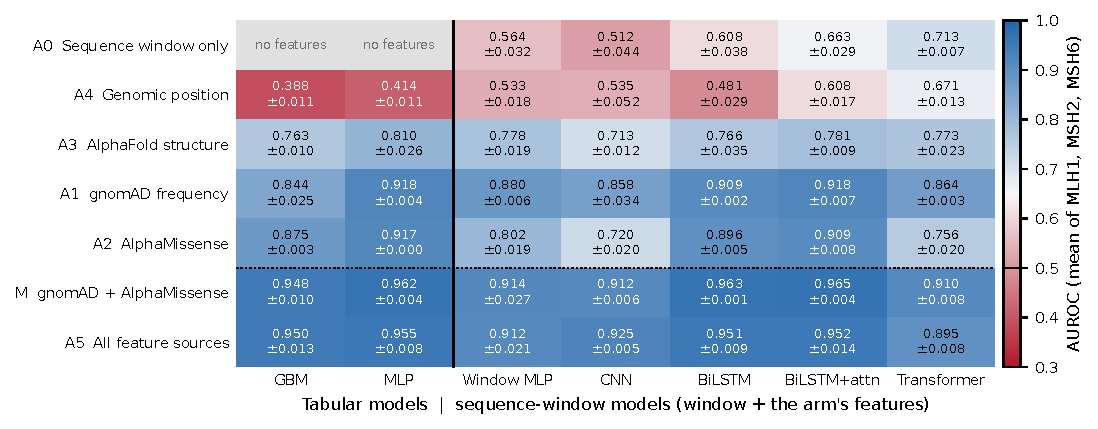
\includegraphics[width=\textwidth]{generated/figures/fig_features.pdf}
\caption{\textbf{Feature sources against architectures.} AUROC (mean over held-out
\gene{MLH1}, \gene{MSH2}, \gene{MSH6}; $\pm$ SD over three seeds) for every feature arm
(rows, ClinVar labels) and model (columns). The tabular models have no input in A0.}
\label{fig:features}
\end{figure}

\begin{table}[t]
\centering
\caption{\textbf{AUROC by feature arm and model} (mean over the three scoreable held-out
genes $\pm$ SD over seeds; best model per arm in bold). MCC is in Supplementary
Table~\ref{tab:supp-arms}.}
\label{tab:features}
\resizebox{\textwidth}{!}{% Generated by paper/analysis.py - do not edit.
\begin{tabular}{llccccccc}
\toprule
Arm & Features & GBM & MLP & Window MLP & CNN & BiLSTM & BiLSTM+attn & Transformer \\
\midrule
A0 & Sequence window only & n/a & n/a & 0.564\,$\pm$\,0.032 & 0.512\,$\pm$\,0.044 & 0.608\,$\pm$\,0.038 & 0.663\,$\pm$\,0.029 & \textbf{0.713\,$\pm$\,0.007} \\
A4 & Genomic position & 0.388\,$\pm$\,0.011 & 0.414\,$\pm$\,0.011 & 0.533\,$\pm$\,0.018 & 0.535\,$\pm$\,0.052 & 0.481\,$\pm$\,0.029 & 0.608\,$\pm$\,0.017 & \textbf{0.671\,$\pm$\,0.013} \\
A3 & AlphaFold structure & 0.763\,$\pm$\,0.010 & \textbf{0.810\,$\pm$\,0.026} & 0.778\,$\pm$\,0.019 & 0.713\,$\pm$\,0.012 & 0.766\,$\pm$\,0.035 & 0.781\,$\pm$\,0.009 & 0.773\,$\pm$\,0.023 \\
A1 & gnomAD frequency & 0.844\,$\pm$\,0.025 & 0.918\,$\pm$\,0.004 & 0.880\,$\pm$\,0.006 & 0.858\,$\pm$\,0.034 & 0.909\,$\pm$\,0.002 & \textbf{0.918\,$\pm$\,0.007} & 0.864\,$\pm$\,0.003 \\
A2 & AlphaMissense & 0.875\,$\pm$\,0.003 & \textbf{0.917\,$\pm$\,0.000} & 0.802\,$\pm$\,0.019 & 0.720\,$\pm$\,0.020 & 0.896\,$\pm$\,0.005 & 0.909\,$\pm$\,0.008 & 0.756\,$\pm$\,0.020 \\
M & gnomAD + AlphaMissense & 0.948\,$\pm$\,0.010 & 0.962\,$\pm$\,0.004 & 0.914\,$\pm$\,0.027 & 0.912\,$\pm$\,0.006 & 0.963\,$\pm$\,0.001 & \textbf{0.965\,$\pm$\,0.004} & 0.910\,$\pm$\,0.008 \\
A5 & All feature sources & 0.950\,$\pm$\,0.013 & \textbf{0.955\,$\pm$\,0.008} & 0.912\,$\pm$\,0.021 & 0.925\,$\pm$\,0.005 & 0.951\,$\pm$\,0.009 & 0.952\,$\pm$\,0.014 & 0.895\,$\pm$\,0.008 \\
\bottomrule
\end{tabular}
}
\end{table}

For the single-feature arms, training can lose information the raw score already has. On
AlphaMissense alone, the MLP reproduces the raw score's ranking (\aucATwoMlp{} against
\baseAlphamissense{} untrained), while GBM's piecewise-constant fit reaches \aucATwoGbm.
On gnomAD alone, GBM reaches \aucAOneGbm{} against \baseNegLogAf{} for the untrained
frequency.

\subsection{Supervision adds little to label-free scores}

The zero-training scores were strong (Figure~\ref{fig:baselines}, Table~\ref{tab:baselines}):
\begin{itemize}
\item $-\log_{10}$ allele frequency: \baseNegLogAf{} \baseCiNegLogAf;
\item AlphaMissense: \baseAlphamissense{} \baseCiAlphamissense;
\item ESM-1b: \baseEsmOneb{} \baseCiEsmOneb;
\item ESM-2: \baseEsmTwo{} \baseCiEsmTwo.
\end{itemize}
In arm M, \nBeatNegLogAfM{} of the 7 trained architectures improved significantly on the
frequency score. The improvements were MLP \dAucMMlpVsNegLogAf, BiLSTM
\dAucMBilstmVsNegLogAf{} and BiLSTM with attention \dAucMBilstmAttnVsNegLogAf. GBM's
interval included zero (\dAucMGbmVsNegLogAf), and the window MLP, CNN and Transformer did
not exceed the untrained score.

The post hoc mean-rank combination of the two scores, which uses no labels, reached
\baseRankMean{} \baseCiRankMean. No trained model exceeded it significantly
(\nBeatRankMeanM{} of 7 in M, \nBeatRankMeanAFive{} of 7 in A5). The closest, BiLSTM with attention
in M, differed by \dAucMBilstmAttnVsRankMean. Because it was constructed after the results
were seen, the combination supports a narrower statement than a pre-specified baseline
would. On this panel, the ClinVar labels of three training genes teach the models little
beyond how to weigh two inputs that are already informative.

\begin{figure}[t]
\centering
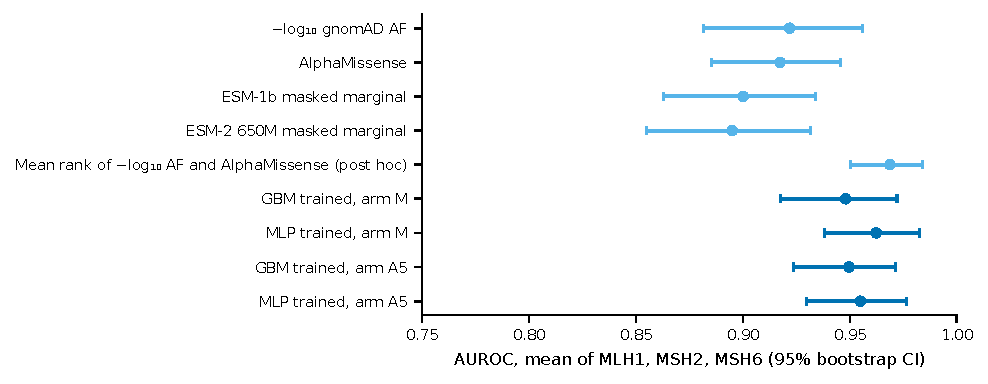
\includegraphics[width=0.78\textwidth]{generated/figures/fig_baselines.pdf}
\caption{\textbf{Zero-training scores against trained models.} AUROC with 95\% bootstrap
intervals over the same held-out variants. Light: scores computed without labels. Dark:
trained GBM and MLP in arms M and A5. The mean-rank combination was added post hoc.}
\label{fig:baselines}
\end{figure}

\begin{table}[t]
\centering
\caption{\textbf{Zero-training scores.} Per-gene AUROC and the mean over genes with a 95\%
bootstrap interval, with trained models for reference.}
\label{tab:baselines}
\resizebox{0.9\textwidth}{!}{% Generated by paper/analysis.py - do not edit.
\begin{tabular}{lcccc}
\toprule
Score (no training on labels) & MLH1 & MSH2 & MSH6 & Mean [95\% CI] \\
\midrule
$-\log_{10}$ gnomAD AF & 0.921 & 0.915 & 0.930 & 0.922 [0.882, 0.956] \\
AlphaMissense & 0.906 & 0.877 & 0.969 & 0.917 [0.885, 0.946] \\
ESM-1b masked marginal & 0.863 & 0.875 & 0.962 & 0.900 [0.863, 0.934] \\
ESM-2 650M masked marginal & 0.837 & 0.898 & 0.950 & 0.895 [0.855, 0.931] \\
Mean rank of $-\log_{10}$ AF and AlphaMissense & 0.967 & 0.956 & 0.983 & 0.969 [0.950, 0.984] \\
\midrule
GBM, gnomAD + AlphaMissense (M) &  &  &  & 0.948 [0.918, 0.972] \\
MLP, gnomAD + AlphaMissense (M) &  &  &  & 0.962 [0.938, 0.982] \\
GBM, All feature sources (A5) &  &  &  & 0.950 [0.924, 0.972] \\
MLP, All feature sources (A5) &  &  &  & 0.955 [0.930, 0.977] \\
\bottomrule
\end{tabular}
}
\end{table}

\subsection{No architecture outperforms gradient boosting}

Within the two strongest feature arms, no sequence-window network had a significantly
higher AUROC than GBM (\nSeqBeatGbmAucM{} of 5 in M, \nSeqBeatGbmAucAFive{} of 5 in
A5). Several were significantly lower (\nSeqWorseGbmAucM{} of 5 in M, \nSeqWorseGbmAucAFive{}
of 5 in A5; Supplementary Table~\ref{tab:model-vs-gbm}). The two BiLSTMs were the closest,
e.g. BiLSTM with attention against GBM in M, \dAucBilstmAttnVsGbmM. The MLP was
indistinguishable from GBM (\dAucMlpVsGbmM). Where the residue window is the only input
(A0), the Transformer does best, and it still reaches only \aucAZeroTransformer. The
window carries some signal on its own, but once frequency and AlphaMissense are present
no window model improved significantly on GBM with the same features.

Seed variation was large for threshold-dependent metrics. The MCC standard deviation over
three seeds reached \maxMccSd{} (\maxMccSdCell), against at most \maxAucSd{} for AUROC.
A single-seed MCC comparison on this panel would be uninterpretable.

\subsection{Labels: expert-panel labels suffice; DMS labels transfer but break thresholds}

Figure~\ref{fig:labels} and Table~\ref{tab:labels} compare each label source with
ClinVar (A5), paired and on identical variants.

\textbf{Expert panel only (B3).} The \nExpert{} expert-panel labels matched all \nLabelled{}
ClinVar labels for the tabular models: GBM \dAucBThreeVsAFiveGbm, MLP
\dAucBThreeVsAFiveMlp. MCC rose slightly for GBM (\dMccBThreeVsAFiveGbm). Among the sequence networks,
\nModelsBThreeAucExcl{} lost AUROC; the largest loss was the Transformer's,
\dAucBThreeVsAFiveTransformer.

\textbf{DMS only (B1).} Labels from one \gene{MSH2} assay transferred to \gene{MLH1} and
\gene{MSH6} with AUROC \aucBOneCnn--\aucBOneGbm. Relative to ClinVar training on the same
genes, the differences ranged from \bOneAucWorst{} to \bOneAucLeast. With all features available, the ranking comes
largely from the features, and the labels mainly orient them.

\textbf{ClinVar + DMS pooled (B2).} Pooling did not change discrimination consistently.
AUROC fell for GBM (\dAucBTwoVsAFiveGbm) and rose for the Transformer
(\dAucBTwoVsAFiveTransformer), and the other \nModelsBTwoAucNull{} intervals included
zero. MCC fell for all \nModelsBTwoMccWorse{} architectures, by \bTwoMccLeast{} to
\bTwoMccWorst, and calibration degraded (GBM Brier score \brierAFiveGbm{} with ClinVar
against \brierBTwoGbm{} pooled). The mechanism is the threshold. In B2 the
inner-validation labels that set it are \valPrevBTwo{} pathogenic, against
\valPrevAFive{} with ClinVar labels and \testPrev{} in the held-out ClinVar genes, so the
selected threshold does not transfer. A pooled model can rank as well as a ClinVar-only
model and still classify worse.

\begin{figure}[t]
\centering
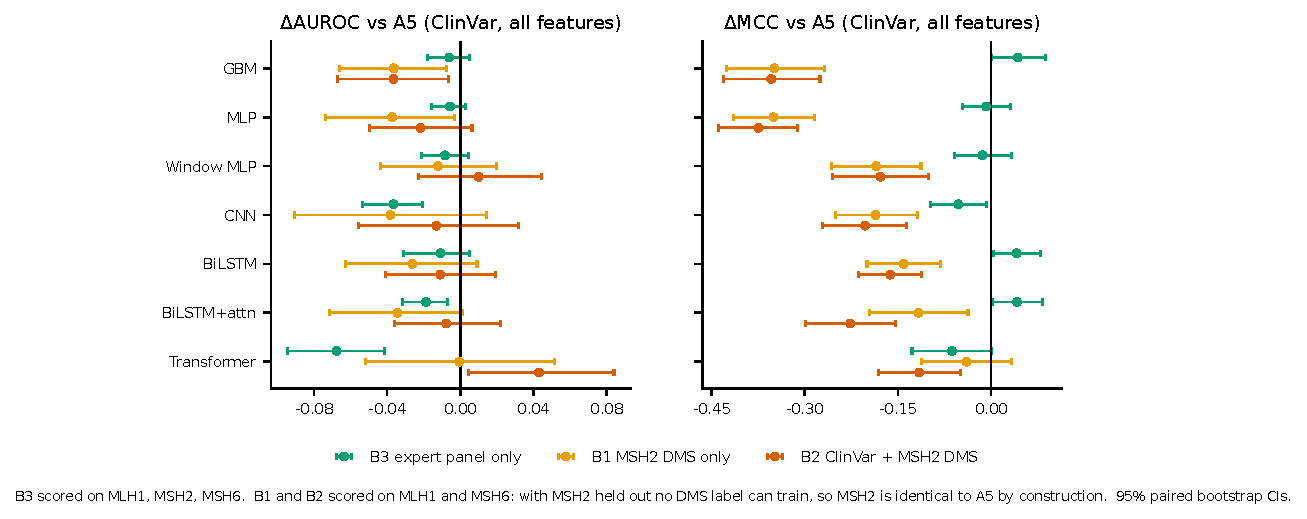
\includegraphics[width=\textwidth]{generated/figures/fig_labels.pdf}
\caption{\textbf{Label sources against ClinVar training (A5), all features.} Paired
$\Delta$AUROC (left) and $\Delta$MCC (right), with 95\% bootstrap intervals. B3 is scored
on \gene{MLH1}, \gene{MSH2} and \gene{MSH6}; B1 and B2 on \gene{MLH1} and \gene{MSH6}, the
genes on which DMS labels can enter training.}
\label{fig:labels}
\end{figure}

\begin{table}[t]
\centering
\caption{\textbf{Label sources against ClinVar training} (A5, all features; paired
difference [95\% CI]; bold: interval excludes zero).}
\label{tab:labels}
\resizebox{\textwidth}{!}{% Generated by paper/analysis.py - do not edit.
\begin{tabular}{lcccccc}
\toprule
 & \multicolumn{2}{c}{B3: expert panel only} & \multicolumn{2}{c}{B1: MSH2 DMS only} & \multicolumn{2}{c}{B2: ClinVar + MSH2 DMS} \\
 & \multicolumn{2}{c}{(MLH1, MSH2, MSH6)} & \multicolumn{2}{c}{(MLH1, MSH6)} & \multicolumn{2}{c}{(MLH1, MSH6)} \\
\cmidrule(lr){2-3}\cmidrule(lr){4-5}\cmidrule(lr){6-7}
Model & $\Delta$AUROC & $\Delta$MCC & $\Delta$AUROC & $\Delta$MCC & $\Delta$AUROC & $\Delta$MCC \\
\midrule
GBM & $-$0.006 [$-$0.018, +0.005] & \textbf{+0.043 [+0.001, +0.087]} & \textbf{$-$0.036 [$-$0.066, $-$0.008]} & \textbf{$-$0.349 [$-$0.425, $-$0.268]} & \textbf{$-$0.037 [$-$0.067, $-$0.006]} & \textbf{$-$0.354 [$-$0.430, $-$0.275]} \\
MLP & $-$0.006 [$-$0.016, +0.003] & $-$0.008 [$-$0.046, +0.031] & \textbf{$-$0.037 [$-$0.074, $-$0.003]} & \textbf{$-$0.350 [$-$0.414, $-$0.285]} & $-$0.022 [$-$0.050, +0.006] & \textbf{$-$0.375 [$-$0.439, $-$0.311]} \\
Window MLP & $-$0.008 [$-$0.021, +0.005] & $-$0.014 [$-$0.059, +0.033] & $-$0.012 [$-$0.044, +0.020] & \textbf{$-$0.185 [$-$0.257, $-$0.113]} & +0.010 [$-$0.023, +0.044] & \textbf{$-$0.178 [$-$0.256, $-$0.101]} \\
CNN & \textbf{$-$0.036 [$-$0.054, $-$0.021]} & \textbf{$-$0.053 [$-$0.097, $-$0.007]} & $-$0.038 [$-$0.091, +0.014] & \textbf{$-$0.186 [$-$0.251, $-$0.119]} & $-$0.013 [$-$0.056, +0.032] & \textbf{$-$0.203 [$-$0.271, $-$0.136]} \\
BiLSTM & $-$0.011 [$-$0.031, +0.005] & \textbf{+0.041 [+0.004, +0.079]} & $-$0.026 [$-$0.063, +0.009] & \textbf{$-$0.141 [$-$0.200, $-$0.082]} & $-$0.011 [$-$0.041, +0.019] & \textbf{$-$0.162 [$-$0.213, $-$0.112]} \\
BiLSTM+attn & \textbf{$-$0.019 [$-$0.032, $-$0.007]} & \textbf{+0.042 [+0.003, +0.083]} & $-$0.034 [$-$0.071, +0.001] & \textbf{$-$0.117 [$-$0.195, $-$0.037]} & $-$0.008 [$-$0.036, +0.022] & \textbf{$-$0.227 [$-$0.299, $-$0.154]} \\
Transformer & \textbf{$-$0.068 [$-$0.095, $-$0.042]} & $-$0.063 [$-$0.127, +0.001] & $-$0.001 [$-$0.052, +0.052] & $-$0.040 [$-$0.112, +0.033] & \textbf{+0.043 [+0.004, +0.084]} & \textbf{$-$0.116 [$-$0.182, $-$0.049]} \\
\bottomrule
\end{tabular}
}
\end{table}

\subsection{How much of the frequency signal is circular?}

Population frequency is both the strongest feature and a criterion used to classify
variants~\citep{richards2015acmg}. It is also the source of AlphaMissense's training
labels~\citep{cheng2023alphamissense}. The simplest version of the circularity is the
presence shortcut: almost every benign variant is observed in gnomAD. We re-scored the
models on the gnomAD-observed variants only (\nObsBenign{} benign, \nObsPath{}
pathogenic), where presence cannot separate the classes
(Figure~\ref{fig:circularity}b, Table~\ref{tab:observed}). Discrimination did not fall:
\begin{itemize}
\item $-\log_{10}$ allele frequency: \aucObsBaselineNegLogAf{} \aucObsCiBaselineNegLogAf;
\item AlphaMissense: \aucObsBaselineAlphamissense;
\item MLP in arm M: \aucObsMMlp.
\end{itemize}
Among observed variants, the frequency level itself still separates the classes, mostly
below the BS1 threshold. This rules out the crudest shortcut. It does not show that the
signal is biological. Curators may weigh sub-threshold frequency informally, and
computational predictions enter classifications as PP3 or BP4
evidence~\citep{pejaver2022pp3}. Where either happened, the ClinVar label is partly a
function of the model inputs, and nothing in a ClinVar-scored design can separate that from
genuine predictive value. Labels that are independent of frequency, such as functional
assays of variants never used in classification or outcome-based evidence, would be
needed.

\begin{figure}[t]
\centering
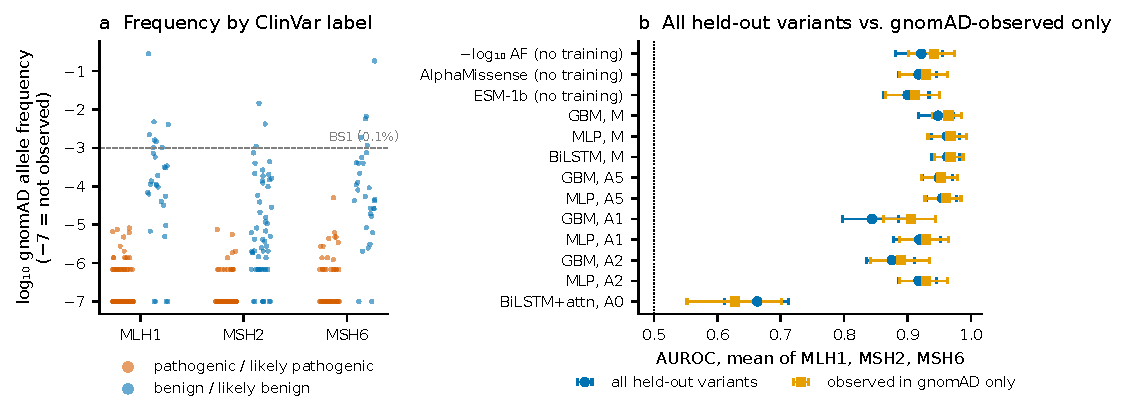
\includegraphics[width=\textwidth]{generated/figures/fig_circularity.pdf}
\caption{\textbf{Frequency and labels.} (a) gnomAD allele frequency of every held-out
ClinVar variant by label ($-7$ = not observed; dashed line, BS1 at 0.1\%). (b) AUROC on
all held-out variants and on the gnomAD-observed variants only, where presence in gnomAD
cannot separate the classes. 95\% bootstrap intervals.}
\label{fig:circularity}
\end{figure}

\begin{table}[t]
\centering
\caption{\textbf{Discrimination without the absent-from-gnomAD shortcut.} AUROC [95\% CI],
mean over \gene{MLH1}, \gene{MSH2}, \gene{MSH6}.}
\label{tab:observed}
\resizebox{0.85\textwidth}{!}{% Generated by paper/analysis.py - do not edit.
\begin{tabular}{lcc}
\toprule
Predictor & All held-out variants & Variants observed in gnomAD \\
\midrule
$-\log_{10}$ gnomAD AF (no training) & 0.922 [0.882, 0.956] & 0.942 [0.902, 0.974] \\
AlphaMissense (no training) & 0.917 [0.885, 0.946] & 0.929 [0.887, 0.963] \\
ESM-1b masked marginal (no training) & 0.900 [0.863, 0.934] & 0.911 [0.865, 0.951] \\
GBM, gnomAD + AlphaMissense (M) & 0.948 [0.918, 0.972] & 0.965 [0.939, 0.985] \\
MLP, gnomAD + AlphaMissense (M) & 0.962 [0.938, 0.982] & 0.968 [0.932, 0.992] \\
BiLSTM, gnomAD + AlphaMissense (M) & 0.963 [0.938, 0.982] & 0.968 [0.943, 0.988] \\
GBM, All feature sources (A5) & 0.950 [0.924, 0.972] & 0.953 [0.922, 0.978] \\
MLP, All feature sources (A5) & 0.955 [0.930, 0.977] & 0.960 [0.928, 0.984] \\
GBM, gnomAD frequency (A1) & 0.844 [0.798, 0.886] & 0.906 [0.862, 0.945] \\
MLP, gnomAD frequency (A1) & 0.918 [0.878, 0.953] & 0.929 [0.887, 0.964] \\
GBM, AlphaMissense (A2) & 0.875 [0.835, 0.910] & 0.890 [0.841, 0.934] \\
MLP, AlphaMissense (A2) & 0.917 [0.885, 0.946] & 0.929 [0.887, 0.963] \\
BiLSTM+attn, Sequence window only (A0) & 0.663 [0.611, 0.713] & 0.628 [0.552, 0.701] \\
\bottomrule
\end{tabular}
}
\end{table}

\subsection{Robustness}

\textbf{Known feature defect.} An audit found that when several nucleotide changes give
the same protein change, the gnomAD frequency feature keeps the first allele's value.
For \nBOne{} labelled variants the feature disagrees with a recount (\nBOneGenes). Removing them changed no
AUROC by more than \bOneMaxChange{} (Supplementary Table~\ref{tab:b1}). The four headline
comparisons we recomputed without them (pooled against ClinVar labels for GBM and MLP;
gnomAD alone, and gnomAD + AlphaMissense, against all sources for GBM) kept their sign.

\textbf{Reproducibility.} Some cells were executed more than once during the grid; the
repeat outputs were archived rather than reported. All \nRepeatIdentical{} of
\nRepeatRuns{} repeated executions produced byte-identical predictions, including across
two code revisions on the GPU.

\textbf{GBM defaults.} GBM with early stopping on the inner-validation set, run in arm M
only, reached \aucMGbmEs. That is a small improvement over the default GBM
(\dAucGbmEsVsGbm) and indistinguishable from the MLP (\dAucGbmEsVsMlp). The comparisons
with GBM above use the default configuration, so they slightly understate it.

% ===========================================================================
\section{Discussion}

The study set out to measure which of the three construction choices matters for
predicting pathogenicity in an unseen Lynch syndrome gene. On this panel the answer is
the features, and specifically two of them. Population frequency and AlphaMissense
together explain almost all the discrimination any model reached. Once those two are
present, structure and genomic position add nothing measurable, and no model reading the
residue window improves on gradient boosting over the same features. No
neural architecture beat gradient boosting. Training on the expert-panel subset alone
(\nExpert{} of \nLabelled{} labels) cost the tabular models nothing. A large pool of functional-assay labels from one gene did not help
ranking consistently, and it did harm classification, through a mechanism that is easy to
miss: the decision threshold is learned on labels whose class balance differs from the
clinical test set.

These results agree with genome-wide observations made with different designs.
AnnotateMissense reports that removing population-frequency and prior-predictor features
reduces performance~\citep{muneeb2026annotatemissense}. Evaluations that remove gene
identity find that much of a ClinVar benchmark score is structure, not variant-level
signal~\citep{harrizi2026geneidentity}. Our leave-one-gene-out design removes gene
identity by construction, and within-gene AUROC remains high. What remains is the
frequency signal, whose relation to the labels we cannot resolve. Our DMS result extends
earlier reports that DMS measurements track clinical pathogenicity~\citep{livesey2020dms}
and can improve clinical prediction when used to train or fine-tune
models~\citep{lafita2024dmsft,jagota2023transfer}. On this panel
DMS labels on their own transferred almost as well as ClinVar labels, but pooling them
with ClinVar in a single classifier harmed classification. How the sources are combined
matters as much as whether they are.

\textbf{Implications.} For a panel of this size we suggest three practices:
\begin{itemize}
\item Report label-free baselines, at least $-\log_{10}$ allele frequency and
  AlphaMissense, on the same variants and split. On our data the frequency score is within
  \dAucMBilstmAttnVsNegLogAfAbs{} AUROC of the best trained model, and a label-free
  combination of the two matches it.
\item Report a threshold-free metric alongside any thresholded one when label sources
  differ.
\item Treat a DMS assay from one gene as a source to be calibrated, not pooled.
\end{itemize}

\textbf{Limitations.}
\begin{itemize}
\item \textbf{Size.} The panel is small: three scoreable genes and \nLabelledScoreable{}
  test variants, so intervals are wide. Each held-out gene's paralogue stays in training,
  so the task is transfer within the MutS and MutL families.
\item \textbf{DMS arms.} The DMS arms rest on a single assay in a single gene, so ``DMS
  labels'' here means ``this \gene{MSH2} assay'' and is confounded with gene identity.
\item \textbf{Circularity.} Both leading features are entangled with how ClinVar labels
  are made, so our AUROCs are upper bounds on what a model would achieve against
  independent truth.
\item \textbf{Hyperparameters.} Defaults were used throughout, never tuned per arm. Tuning
  could favour the neural models more than the trees, although the zero-training results
  leave little room above them.
\item \textbf{Calibration.} The neural models use class-weighted losses, so their raw
  probabilities are not calibrated to prevalence~\citep{guo2017calibration}. Brier score
  and ECE partly measure that weighting.
\item \textbf{Frequency flags.} The ACMG flags use generic thresholds, not the InSiGHT
  expert panel's gene-specific specification. The continuous frequency feature is
  present in every gnomAD arm regardless.
\item \textbf{ClinVar version.} ClinVar is a single snapshot (downloaded 28 August 2026).
  Classifications change over time, and a temporal hold-out would test a different
  question.
\end{itemize}

% ===========================================================================
\section{Conclusion}

For cross-gene pathogenicity prediction in the Lynch syndrome MMR genes, population
frequency and AlphaMissense account for nearly all the discrimination that seven
architectures and four label sources achieve. The large neural models, the extra
structural features and the extra functional-assay labels bought nothing measurable in
ranking, and the pooled labels made classification worse. The question left open is
whether the frequency signal reflects biology or the way the labels were made. On ClinVar
labels alone it cannot be answered.

% ===========================================================================
\section*{Data and code availability}
Everything needed to reproduce this paper is in the repository
(\url{https://github.com/jvikramsrd/variant_pathogenicity_dl}):
\begin{itemize}
\item the variant table (\texttt{data/built/canonical\_full.csv});
\item the ablation script (\texttt{scripts/dl\_ablation.sh});
\item the per-variant predictions, inner-validation predictions and run summaries of every
  run (\texttt{runs/dl/});
\item the run-level summary (\texttt{results/dl/});
\item the analysis that regenerates every number, table and figure
  (\texttt{paper/analysis.py}).
\end{itemize}
Each run records the dataset hash, the split hash, the feature-schema hash, the git
commit and the library versions. The source data are public: ClinVar (public domain),
gnomAD (CC0), AlphaMissense (CC~BY~4.0), AlphaFold DB (CC~BY~4.0), ProteinGym (MIT) and
UniProt (CC~BY~4.0). \todo{Archive the repository (e.g.\ Zenodo) and give the DOI.}

\section*{Acknowledgements}
\todo{Acknowledgements.}

\section*{Funding}
\todo{Funding statement.}

\section*{Conflict of interest}
\todo{Declaration.}

\bibliographystyle{unsrtnat}
\bibliography{references}

% ===========================================================================
\clearpage
\appendix
\renewcommand{\thetable}{S\arabic{table}}
\renewcommand{\thefigure}{S\arabic{figure}}
\setcounter{table}{0}
\setcounter{figure}{0}
\section*{Supplementary material}

\begin{figure}[h]
\centering
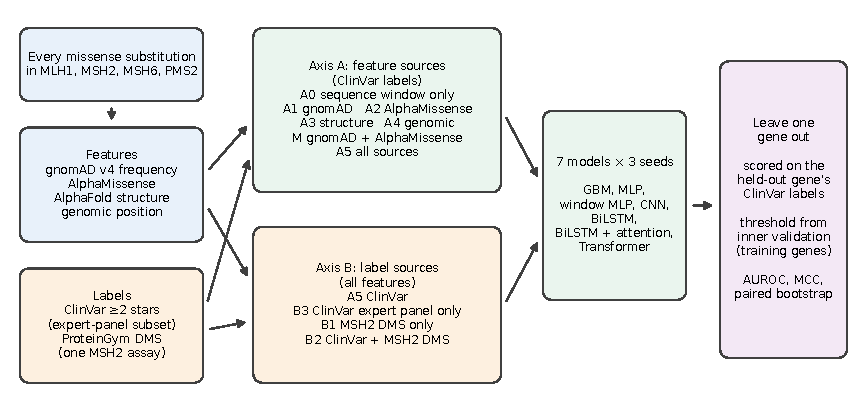
\includegraphics[width=\textwidth]{generated/figures/fig_design.pdf}
\caption{\textbf{Study design.} Axis A varies the feature sources of a ClinVar-trained
model. Axis B varies the label sources with all features. Every arm is run with seven
models and three seeds and scored leave-one-gene-out on the held-out gene's ClinVar
labels. The decision threshold comes from inner validation on the training genes.}
\label{fig:design}
\end{figure}

\begin{figure}[h]
\centering
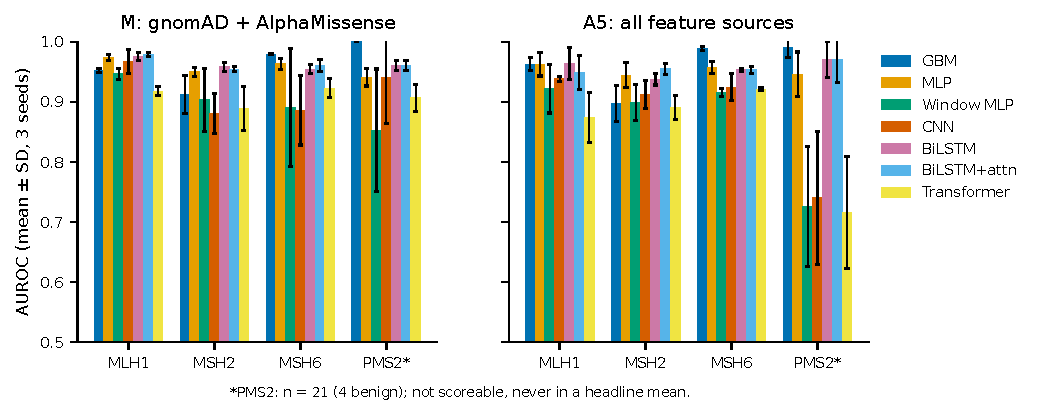
\includegraphics[width=\textwidth]{generated/figures/fig_per_gene.pdf}
\caption{\textbf{AUROC per held-out gene} for arms M and A5 (mean $\pm$ SD over three
seeds).}
\label{fig:per-gene}
\end{figure}

\begin{table}[h]
\centering
\caption{\textbf{Architectures against GBM} within arms M and A5 (paired difference
[95\% CI]; bold: interval excludes zero).}
\label{tab:model-vs-gbm}
\resizebox{\textwidth}{!}{% Generated by paper/analysis.py - do not edit.
\begin{tabular}{lcccc}
\toprule
 & \multicolumn{2}{c}{M: gnomAD + AlphaMissense} & \multicolumn{2}{c}{A5: all feature sources} \\
\cmidrule(lr){2-3}\cmidrule(lr){4-5}
Model & $\Delta$AUROC & $\Delta$MCC & $\Delta$AUROC & $\Delta$MCC \\
\midrule
MLP & +0.014 [$-$0.001, +0.031] & +0.023 [$-$0.004, +0.051] & +0.005 [$-$0.011, +0.021] & \textbf{$-$0.056 [$-$0.098, $-$0.013]} \\
Window MLP & \textbf{$-$0.034 [$-$0.058, $-$0.010]} & \textbf{$-$0.174 [$-$0.226, $-$0.119]} & \textbf{$-$0.037 [$-$0.063, $-$0.011]} & \textbf{$-$0.185 [$-$0.245, $-$0.129]} \\
CNN & \textbf{$-$0.036 [$-$0.064, $-$0.010]} & \textbf{$-$0.130 [$-$0.191, $-$0.069]} & $-$0.024 [$-$0.051, +0.002] & \textbf{$-$0.198 [$-$0.251, $-$0.145]} \\
BiLSTM & +0.015 [$-$0.004, +0.035] & $-$0.003 [$-$0.042, +0.037] & +0.002 [$-$0.018, +0.021] & \textbf{$-$0.170 [$-$0.226, $-$0.112]} \\
BiLSTM+attn & +0.017 [$-$0.001, +0.036] & $-$0.005 [$-$0.044, +0.033] & +0.003 [$-$0.016, +0.022] & \textbf{$-$0.129 [$-$0.184, $-$0.072]} \\
Transformer & \textbf{$-$0.038 [$-$0.072, $-$0.002]} & \textbf{$-$0.130 [$-$0.199, $-$0.062]} & \textbf{$-$0.054 [$-$0.087, $-$0.023]} & \textbf{$-$0.238 [$-$0.304, $-$0.172]} \\
\bottomrule
\end{tabular}
}
\end{table}

\begin{table}[h]
\centering
\caption{\textbf{Each feature arm against all sources (A5)}, paired $\Delta$AUROC (bold:
95\% interval excludes zero).}
\label{tab:feature-deltas}
\resizebox{\textwidth}{!}{% Generated by paper/analysis.py - do not edit.
\begin{tabular}{lccccccc}
\toprule
Arm $-$ A5 & GBM & MLP & Window MLP & CNN & BiLSTM & BiLSTM+attn & Transformer \\
\midrule
A1 gnomAD & \textbf{$-$0.106} & \textbf{$-$0.036} & \textbf{$-$0.033} & \textbf{$-$0.067} & \textbf{$-$0.043} & \textbf{$-$0.034} & \textbf{$-$0.031} \\
A2 AlphaMissense & \textbf{$-$0.074} & \textbf{$-$0.038} & \textbf{$-$0.111} & \textbf{$-$0.205} & \textbf{$-$0.055} & \textbf{$-$0.044} & \textbf{$-$0.139} \\
A3 structure & \textbf{$-$0.187} & \textbf{$-$0.145} & \textbf{$-$0.135} & \textbf{$-$0.213} & \textbf{$-$0.185} & \textbf{$-$0.171} & \textbf{$-$0.123} \\
A4 genomic & \textbf{$-$0.562} & \textbf{$-$0.541} & \textbf{$-$0.379} & \textbf{$-$0.390} & \textbf{$-$0.470} & \textbf{$-$0.344} & \textbf{$-$0.225} \\
M gnomAD + AlphaMissense & $-$0.002 & +0.007 & +0.001 & $-$0.014 & +0.011 & +0.012 & +0.015 \\
\bottomrule
\end{tabular}
}
\end{table}

\begin{table}[h]
\centering
\caption{\textbf{MCC by feature arm and model} (mean $\pm$ SD over seeds; threshold from
inner validation).}
\label{tab:features-mcc}
\resizebox{\textwidth}{!}{% Generated by paper/analysis.py - do not edit.
\begin{tabular}{llccccccc}
\toprule
Arm & Features & GBM & MLP & Window MLP & CNN & BiLSTM & BiLSTM+attn & Transformer \\
\midrule
A0 & Sequence window only & n/a & n/a & 0.103\,$\pm$\,0.029 & 0.018\,$\pm$\,0.073 & 0.095\,$\pm$\,0.088 & 0.180\,$\pm$\,0.013 & \textbf{0.220\,$\pm$\,0.059} \\
A4 & Genomic position & -0.094\,$\pm$\,0.090 & -0.032\,$\pm$\,0.093 & 0.018\,$\pm$\,0.038 & 0.020\,$\pm$\,0.048 & 0.067\,$\pm$\,0.075 & 0.150\,$\pm$\,0.044 & \textbf{0.189\,$\pm$\,0.027} \\
A3 & AlphaFold structure & 0.392\,$\pm$\,0.054 & \textbf{0.396\,$\pm$\,0.120} & 0.359\,$\pm$\,0.063 & 0.264\,$\pm$\,0.059 & 0.282\,$\pm$\,0.018 & 0.375\,$\pm$\,0.034 & 0.365\,$\pm$\,0.055 \\
A1 & gnomAD frequency & 0.655\,$\pm$\,0.031 & \textbf{0.686\,$\pm$\,0.047} & 0.538\,$\pm$\,0.052 & 0.515\,$\pm$\,0.144 & 0.656\,$\pm$\,0.058 & 0.683\,$\pm$\,0.049 & 0.486\,$\pm$\,0.032 \\
A2 & AlphaMissense & 0.546\,$\pm$\,0.032 & \textbf{0.623\,$\pm$\,0.021} & 0.394\,$\pm$\,0.014 & 0.270\,$\pm$\,0.026 & 0.609\,$\pm$\,0.049 & 0.572\,$\pm$\,0.036 & 0.306\,$\pm$\,0.065 \\
M & gnomAD + AlphaMissense & 0.776\,$\pm$\,0.051 & \textbf{0.799\,$\pm$\,0.006} & 0.602\,$\pm$\,0.074 & 0.646\,$\pm$\,0.067 & 0.773\,$\pm$\,0.042 & 0.770\,$\pm$\,0.028 & 0.645\,$\pm$\,0.043 \\
A5 & All feature sources & \textbf{0.743\,$\pm$\,0.023} & 0.687\,$\pm$\,0.151 & 0.558\,$\pm$\,0.043 & 0.545\,$\pm$\,0.106 & 0.573\,$\pm$\,0.067 & 0.614\,$\pm$\,0.129 & 0.505\,$\pm$\,0.090 \\
\bottomrule
\end{tabular}
}
\end{table}

\begin{table}[h]
\centering
\caption{\textbf{Sensitivity to the gnomAD allele-collapsing defect.} AUROC with and
without the \nBOne{} labelled variants whose frequency feature disagrees with a recount.}
\label{tab:b1}
% Generated by paper/analysis.py - do not edit.
\begin{tabular}{lccc}
\toprule
Cell & AUROC, all & AUROC, affected variants removed & Change \\
\midrule
MLP, gnomAD + AlphaMissense (M) & 0.962 & 0.964 & +0.001 \\
GBM, gnomAD + AlphaMissense (M) & 0.948 & 0.952 & +0.004 \\
GBM, All feature sources (A5) & 0.950 & 0.952 & +0.003 \\
MLP, All feature sources (A5) & 0.955 & 0.957 & +0.002 \\
GBM, gnomAD frequency (A1) & 0.844 & 0.851 & +0.007 \\
\bottomrule
\end{tabular}

\end{table}

{\small
% Generated by paper/analysis.py - do not edit.
\begin{longtable}{llllccccc}
\caption{Every arm and model: mean over the held-out genes listed, $\pm$ SD over three seeds. Brier score and ECE are reported as trained; the models use class-weighted losses, so these measure the weighting as well as the model.}\label{tab:supp-arms}\\
\toprule
Arm & Model & Held-out genes & AUROC & MCC & PR-AUC & Brier & ECE \\
\midrule
\endfirsthead
\toprule
Arm & Model & Held-out genes & AUROC & MCC & PR-AUC & Brier & ECE \\
\midrule
\endhead
A0 & Window MLP & MLH1, MSH2, MSH6 & 0.564\,$\pm$\,0.032 & 0.103\,$\pm$\,0.029 & 0.754\,$\pm$\,0.021 & 0.333\,$\pm$\,0.023 & 0.325\,$\pm$\,0.002 \\
A0 & CNN & MLH1, MSH2, MSH6 & 0.512\,$\pm$\,0.044 & 0.018\,$\pm$\,0.073 & 0.719\,$\pm$\,0.022 & 0.374\,$\pm$\,0.045 & 0.372\,$\pm$\,0.051 \\
A0 & BiLSTM & MLH1, MSH2, MSH6 & 0.608\,$\pm$\,0.038 & 0.095\,$\pm$\,0.088 & 0.797\,$\pm$\,0.016 & 0.300\,$\pm$\,0.019 & 0.312\,$\pm$\,0.032 \\
A0 & BiLSTM+attn & MLH1, MSH2, MSH6 & 0.663\,$\pm$\,0.029 & 0.180\,$\pm$\,0.013 & 0.830\,$\pm$\,0.014 & 0.263\,$\pm$\,0.030 & 0.240\,$\pm$\,0.032 \\
A0 & Transformer & MLH1, MSH2, MSH6 & 0.713\,$\pm$\,0.007 & 0.220\,$\pm$\,0.059 & 0.854\,$\pm$\,0.001 & 0.262\,$\pm$\,0.028 & 0.254\,$\pm$\,0.042 \\
A1 & GBM & MLH1, MSH2, MSH6 & 0.844\,$\pm$\,0.025 & 0.655\,$\pm$\,0.031 & 0.888\,$\pm$\,0.014 & 0.110\,$\pm$\,0.003 & 0.104\,$\pm$\,0.005 \\
A1 & MLP & MLH1, MSH2, MSH6 & 0.918\,$\pm$\,0.004 & 0.686\,$\pm$\,0.047 & 0.947\,$\pm$\,0.001 & 0.126\,$\pm$\,0.019 & 0.158\,$\pm$\,0.009 \\
A1 & Window MLP & MLH1, MSH2, MSH6 & 0.880\,$\pm$\,0.006 & 0.538\,$\pm$\,0.052 & 0.930\,$\pm$\,0.008 & 0.163\,$\pm$\,0.008 & 0.192\,$\pm$\,0.006 \\
A1 & CNN & MLH1, MSH2, MSH6 & 0.858\,$\pm$\,0.034 & 0.515\,$\pm$\,0.144 & 0.902\,$\pm$\,0.023 & 0.225\,$\pm$\,0.022 & 0.277\,$\pm$\,0.025 \\
A1 & BiLSTM & MLH1, MSH2, MSH6 & 0.909\,$\pm$\,0.002 & 0.656\,$\pm$\,0.058 & 0.928\,$\pm$\,0.009 & 0.136\,$\pm$\,0.015 & 0.166\,$\pm$\,0.025 \\
A1 & BiLSTM+attn & MLH1, MSH2, MSH6 & 0.918\,$\pm$\,0.007 & 0.683\,$\pm$\,0.049 & 0.939\,$\pm$\,0.012 & 0.129\,$\pm$\,0.022 & 0.168\,$\pm$\,0.054 \\
A1 & Transformer & MLH1, MSH2, MSH6 & 0.864\,$\pm$\,0.003 & 0.486\,$\pm$\,0.032 & 0.925\,$\pm$\,0.006 & 0.148\,$\pm$\,0.009 & 0.139\,$\pm$\,0.015 \\
A2 & GBM & MLH1, MSH2, MSH6 & 0.875\,$\pm$\,0.003 & 0.546\,$\pm$\,0.032 & 0.932\,$\pm$\,0.015 & 0.121\,$\pm$\,0.002 & 0.108\,$\pm$\,0.005 \\
A2 & MLP & MLH1, MSH2, MSH6 & 0.917\,$\pm$\,0.000 & 0.623\,$\pm$\,0.021 & 0.958\,$\pm$\,0.000 & 0.110\,$\pm$\,0.006 & 0.121\,$\pm$\,0.020 \\
A2 & Window MLP & MLH1, MSH2, MSH6 & 0.802\,$\pm$\,0.019 & 0.394\,$\pm$\,0.014 & 0.904\,$\pm$\,0.012 & 0.206\,$\pm$\,0.010 & 0.204\,$\pm$\,0.026 \\
A2 & CNN & MLH1, MSH2, MSH6 & 0.720\,$\pm$\,0.020 & 0.270\,$\pm$\,0.026 & 0.843\,$\pm$\,0.031 & 0.244\,$\pm$\,0.020 & 0.241\,$\pm$\,0.036 \\
A2 & BiLSTM & MLH1, MSH2, MSH6 & 0.896\,$\pm$\,0.005 & 0.609\,$\pm$\,0.049 & 0.952\,$\pm$\,0.002 & 0.129\,$\pm$\,0.003 & 0.140\,$\pm$\,0.020 \\
A2 & BiLSTM+attn & MLH1, MSH2, MSH6 & 0.909\,$\pm$\,0.008 & 0.572\,$\pm$\,0.036 & 0.960\,$\pm$\,0.004 & 0.119\,$\pm$\,0.003 & 0.126\,$\pm$\,0.008 \\
A2 & Transformer & MLH1, MSH2, MSH6 & 0.756\,$\pm$\,0.020 & 0.306\,$\pm$\,0.065 & 0.882\,$\pm$\,0.014 & 0.231\,$\pm$\,0.024 & 0.214\,$\pm$\,0.029 \\
A3 & GBM & MLH1, MSH2, MSH6 & 0.763\,$\pm$\,0.010 & 0.392\,$\pm$\,0.054 & 0.856\,$\pm$\,0.008 & 0.182\,$\pm$\,0.010 & 0.162\,$\pm$\,0.006 \\
A3 & MLP & MLH1, MSH2, MSH6 & 0.810\,$\pm$\,0.026 & 0.396\,$\pm$\,0.120 & 0.898\,$\pm$\,0.025 & 0.182\,$\pm$\,0.007 & 0.181\,$\pm$\,0.013 \\
A3 & Window MLP & MLH1, MSH2, MSH6 & 0.778\,$\pm$\,0.019 & 0.359\,$\pm$\,0.063 & 0.890\,$\pm$\,0.019 & 0.204\,$\pm$\,0.002 & 0.187\,$\pm$\,0.038 \\
A3 & CNN & MLH1, MSH2, MSH6 & 0.713\,$\pm$\,0.012 & 0.264\,$\pm$\,0.059 & 0.845\,$\pm$\,0.008 & 0.235\,$\pm$\,0.012 & 0.237\,$\pm$\,0.031 \\
A3 & BiLSTM & MLH1, MSH2, MSH6 & 0.766\,$\pm$\,0.035 & 0.282\,$\pm$\,0.018 & 0.881\,$\pm$\,0.018 & 0.205\,$\pm$\,0.015 & 0.185\,$\pm$\,0.014 \\
A3 & BiLSTM+attn & MLH1, MSH2, MSH6 & 0.781\,$\pm$\,0.009 & 0.375\,$\pm$\,0.034 & 0.890\,$\pm$\,0.014 & 0.212\,$\pm$\,0.009 & 0.206\,$\pm$\,0.006 \\
A3 & Transformer & MLH1, MSH2, MSH6 & 0.773\,$\pm$\,0.023 & 0.365\,$\pm$\,0.055 & 0.888\,$\pm$\,0.009 & 0.208\,$\pm$\,0.038 & 0.196\,$\pm$\,0.037 \\
A4 & GBM & MLH1, MSH2, MSH6 & 0.388\,$\pm$\,0.011 & -0.094\,$\pm$\,0.090 & 0.652\,$\pm$\,0.010 & 0.352\,$\pm$\,0.005 & 0.364\,$\pm$\,0.019 \\
A4 & MLP & MLH1, MSH2, MSH6 & 0.414\,$\pm$\,0.011 & -0.032\,$\pm$\,0.093 & 0.711\,$\pm$\,0.006 & 0.299\,$\pm$\,0.013 & 0.299\,$\pm$\,0.030 \\
A4 & Window MLP & MLH1, MSH2, MSH6 & 0.533\,$\pm$\,0.018 & 0.018\,$\pm$\,0.038 & 0.733\,$\pm$\,0.007 & 0.307\,$\pm$\,0.015 & 0.314\,$\pm$\,0.006 \\
A4 & CNN & MLH1, MSH2, MSH6 & 0.535\,$\pm$\,0.052 & 0.020\,$\pm$\,0.048 & 0.754\,$\pm$\,0.030 & 0.370\,$\pm$\,0.020 & 0.390\,$\pm$\,0.020 \\
A4 & BiLSTM & MLH1, MSH2, MSH6 & 0.481\,$\pm$\,0.029 & 0.067\,$\pm$\,0.075 & 0.734\,$\pm$\,0.005 & 0.331\,$\pm$\,0.025 & 0.317\,$\pm$\,0.057 \\
A4 & BiLSTM+attn & MLH1, MSH2, MSH6 & 0.608\,$\pm$\,0.017 & 0.150\,$\pm$\,0.044 & 0.799\,$\pm$\,0.011 & 0.349\,$\pm$\,0.019 & 0.342\,$\pm$\,0.017 \\
A4 & Transformer & MLH1, MSH2, MSH6 & 0.671\,$\pm$\,0.013 & 0.189\,$\pm$\,0.027 & 0.839\,$\pm$\,0.010 & 0.281\,$\pm$\,0.011 & 0.257\,$\pm$\,0.018 \\
M & GBM & MLH1, MSH2, MSH6 & 0.948\,$\pm$\,0.010 & 0.776\,$\pm$\,0.051 & 0.962\,$\pm$\,0.011 & 0.074\,$\pm$\,0.004 & 0.080\,$\pm$\,0.005 \\
M & MLP & MLH1, MSH2, MSH6 & 0.962\,$\pm$\,0.004 & 0.799\,$\pm$\,0.006 & 0.978\,$\pm$\,0.007 & 0.076\,$\pm$\,0.014 & 0.107\,$\pm$\,0.036 \\
M & Window MLP & MLH1, MSH2, MSH6 & 0.914\,$\pm$\,0.027 & 0.602\,$\pm$\,0.074 & 0.955\,$\pm$\,0.011 & 0.166\,$\pm$\,0.009 & 0.238\,$\pm$\,0.016 \\
M & CNN & MLH1, MSH2, MSH6 & 0.912\,$\pm$\,0.006 & 0.646\,$\pm$\,0.067 & 0.946\,$\pm$\,0.010 & 0.217\,$\pm$\,0.027 & 0.283\,$\pm$\,0.060 \\
M & BiLSTM & MLH1, MSH2, MSH6 & 0.963\,$\pm$\,0.001 & 0.773\,$\pm$\,0.042 & 0.978\,$\pm$\,0.003 & 0.093\,$\pm$\,0.009 & 0.134\,$\pm$\,0.017 \\
M & BiLSTM+attn & MLH1, MSH2, MSH6 & 0.965\,$\pm$\,0.004 & 0.770\,$\pm$\,0.028 & 0.978\,$\pm$\,0.002 & 0.089\,$\pm$\,0.004 & 0.122\,$\pm$\,0.015 \\
M & Transformer & MLH1, MSH2, MSH6 & 0.910\,$\pm$\,0.008 & 0.645\,$\pm$\,0.043 & 0.948\,$\pm$\,0.006 & 0.132\,$\pm$\,0.004 & 0.141\,$\pm$\,0.007 \\
A5 & GBM & MLH1, MSH2, MSH6 & 0.950\,$\pm$\,0.013 & 0.743\,$\pm$\,0.023 & 0.968\,$\pm$\,0.013 & 0.071\,$\pm$\,0.005 & 0.079\,$\pm$\,0.003 \\
A5 & MLP & MLH1, MSH2, MSH6 & 0.955\,$\pm$\,0.008 & 0.687\,$\pm$\,0.151 & 0.973\,$\pm$\,0.008 & 0.084\,$\pm$\,0.023 & 0.110\,$\pm$\,0.055 \\
A5 & Window MLP & MLH1, MSH2, MSH6 & 0.912\,$\pm$\,0.021 & 0.558\,$\pm$\,0.043 & 0.959\,$\pm$\,0.007 & 0.162\,$\pm$\,0.028 & 0.209\,$\pm$\,0.041 \\
A5 & CNN & MLH1, MSH2, MSH6 & 0.925\,$\pm$\,0.005 & 0.545\,$\pm$\,0.106 & 0.957\,$\pm$\,0.003 & 0.191\,$\pm$\,0.072 & 0.232\,$\pm$\,0.102 \\
A5 & BiLSTM & MLH1, MSH2, MSH6 & 0.951\,$\pm$\,0.009 & 0.573\,$\pm$\,0.067 & 0.973\,$\pm$\,0.003 & 0.135\,$\pm$\,0.031 & 0.187\,$\pm$\,0.040 \\
A5 & BiLSTM+attn & MLH1, MSH2, MSH6 & 0.952\,$\pm$\,0.014 & 0.614\,$\pm$\,0.129 & 0.973\,$\pm$\,0.007 & 0.133\,$\pm$\,0.001 & 0.192\,$\pm$\,0.012 \\
A5 & Transformer & MLH1, MSH2, MSH6 & 0.895\,$\pm$\,0.008 & 0.505\,$\pm$\,0.090 & 0.949\,$\pm$\,0.002 & 0.168\,$\pm$\,0.022 & 0.196\,$\pm$\,0.024 \\
B3 & GBM & MLH1, MSH2, MSH6 & 0.944\,$\pm$\,0.004 & 0.786\,$\pm$\,0.017 & 0.955\,$\pm$\,0.006 & 0.064\,$\pm$\,0.002 & 0.064\,$\pm$\,0.010 \\
B3 & MLP & MLH1, MSH2, MSH6 & 0.949\,$\pm$\,0.005 & 0.680\,$\pm$\,0.048 & 0.974\,$\pm$\,0.003 & 0.110\,$\pm$\,0.017 & 0.178\,$\pm$\,0.047 \\
B3 & Window MLP & MLH1, MSH2, MSH6 & 0.904\,$\pm$\,0.013 & 0.543\,$\pm$\,0.076 & 0.953\,$\pm$\,0.010 & 0.165\,$\pm$\,0.023 & 0.219\,$\pm$\,0.025 \\
B3 & CNN & MLH1, MSH2, MSH6 & 0.889\,$\pm$\,0.026 & 0.492\,$\pm$\,0.034 & 0.941\,$\pm$\,0.021 & 0.209\,$\pm$\,0.024 & 0.263\,$\pm$\,0.042 \\
B3 & BiLSTM & MLH1, MSH2, MSH6 & 0.941\,$\pm$\,0.007 & 0.614\,$\pm$\,0.025 & 0.964\,$\pm$\,0.010 & 0.131\,$\pm$\,0.005 & 0.194\,$\pm$\,0.028 \\
B3 & BiLSTM+attn & MLH1, MSH2, MSH6 & 0.934\,$\pm$\,0.024 & 0.656\,$\pm$\,0.092 & 0.968\,$\pm$\,0.006 & 0.156\,$\pm$\,0.015 & 0.236\,$\pm$\,0.014 \\
B3 & Transformer & MLH1, MSH2, MSH6 & 0.828\,$\pm$\,0.025 & 0.442\,$\pm$\,0.061 & 0.920\,$\pm$\,0.008 & 0.188\,$\pm$\,0.007 & 0.198\,$\pm$\,0.011 \\
B1 & GBM & MLH1, MSH6 & 0.939\,$\pm$\,0.003 & 0.427\,$\pm$\,0.050 & 0.979\,$\pm$\,0.001 & 0.360\,$\pm$\,0.004 & 0.461\,$\pm$\,0.003 \\
B1 & MLP & MLH1, MSH6 & 0.923\,$\pm$\,0.010 & 0.288\,$\pm$\,0.007 & 0.970\,$\pm$\,0.005 & 0.224\,$\pm$\,0.013 & 0.310\,$\pm$\,0.011 \\
B1 & Window MLP & MLH1, MSH6 & 0.907\,$\pm$\,0.030 & 0.397\,$\pm$\,0.181 & 0.970\,$\pm$\,0.008 & 0.231\,$\pm$\,0.050 & 0.305\,$\pm$\,0.043 \\
B1 & CNN & MLH1, MSH6 & 0.893\,$\pm$\,0.005 & 0.369\,$\pm$\,0.021 & 0.964\,$\pm$\,0.002 & 0.184\,$\pm$\,0.013 & 0.244\,$\pm$\,0.008 \\
B1 & BiLSTM & MLH1, MSH6 & 0.932\,$\pm$\,0.010 & 0.393\,$\pm$\,0.110 & 0.974\,$\pm$\,0.003 & 0.182\,$\pm$\,0.023 & 0.263\,$\pm$\,0.040 \\
B1 & BiLSTM+attn & MLH1, MSH6 & 0.917\,$\pm$\,0.030 & 0.480\,$\pm$\,0.055 & 0.972\,$\pm$\,0.009 & 0.210\,$\pm$\,0.038 & 0.291\,$\pm$\,0.052 \\
B1 & Transformer & MLH1, MSH6 & 0.897\,$\pm$\,0.013 & 0.443\,$\pm$\,0.096 & 0.964\,$\pm$\,0.004 & 0.239\,$\pm$\,0.016 & 0.317\,$\pm$\,0.016 \\
B2 & GBM & MLH1, MSH2, MSH6 & 0.925\,$\pm$\,0.006 & 0.507\,$\pm$\,0.048 & 0.960\,$\pm$\,0.008 & 0.255\,$\pm$\,0.004 & 0.328\,$\pm$\,0.007 \\
B2 & MLP & MLH1, MSH2, MSH6 & 0.940\,$\pm$\,0.014 & 0.437\,$\pm$\,0.036 & 0.971\,$\pm$\,0.010 & 0.154\,$\pm$\,0.014 & 0.216\,$\pm$\,0.028 \\
B2 & Window MLP & MLH1, MSH2, MSH6 & 0.919\,$\pm$\,0.005 & 0.439\,$\pm$\,0.034 & 0.967\,$\pm$\,0.001 & 0.199\,$\pm$\,0.018 & 0.244\,$\pm$\,0.024 \\
B2 & CNN & MLH1, MSH2, MSH6 & 0.916\,$\pm$\,0.014 & 0.410\,$\pm$\,0.029 & 0.957\,$\pm$\,0.007 & 0.175\,$\pm$\,0.019 & 0.209\,$\pm$\,0.026 \\
B2 & BiLSTM & MLH1, MSH2, MSH6 & 0.944\,$\pm$\,0.006 & 0.465\,$\pm$\,0.032 & 0.975\,$\pm$\,0.001 & 0.152\,$\pm$\,0.004 & 0.204\,$\pm$\,0.004 \\
B2 & BiLSTM+attn & MLH1, MSH2, MSH6 & 0.947\,$\pm$\,0.006 & 0.463\,$\pm$\,0.081 & 0.976\,$\pm$\,0.005 & 0.170\,$\pm$\,0.022 & 0.235\,$\pm$\,0.028 \\
B2 & Transformer & MLH1, MSH2, MSH6 & 0.924\,$\pm$\,0.006 & 0.428\,$\pm$\,0.058 & 0.965\,$\pm$\,0.005 & 0.199\,$\pm$\,0.002 & 0.252\,$\pm$\,0.003 \\
\bottomrule
\end{longtable}

% Generated by paper/analysis.py - do not edit.
\begin{longtable}{llcccc}
\caption{AUROC per held-out gene (mean $\pm$ SD over three seeds). PMS2 ($n$=21, 4 benign) is reported but never enters a headline mean.}\label{tab:supp-per-gene}\\
\toprule
Arm & Model & MLH1 ($n$=174) & MSH2 ($n$=176) & MSH6 ($n$=78) & PMS2 ($n$=21) \\
\midrule
\endfirsthead
\toprule
Arm & Model & MLH1 ($n$=174) & MSH2 ($n$=176) & MSH6 ($n$=78) & PMS2 ($n$=21) \\
\midrule
\endhead
A0 & Window MLP & 0.582\,$\pm$\,0.049 & 0.597\,$\pm$\,0.052 & 0.513\,$\pm$\,0.036 & 0.554\,$\pm$\,0.098 \\
A0 & CNN & 0.543\,$\pm$\,0.083 & 0.472\,$\pm$\,0.035 & 0.519\,$\pm$\,0.025 & 0.779\,$\pm$\,0.170 \\
A0 & BiLSTM & 0.587\,$\pm$\,0.051 & 0.584\,$\pm$\,0.039 & 0.654\,$\pm$\,0.055 & 0.348\,$\pm$\,0.066 \\
A0 & BiLSTM+attn & 0.661\,$\pm$\,0.017 & 0.646\,$\pm$\,0.014 & 0.682\,$\pm$\,0.079 & 0.441\,$\pm$\,0.029 \\
A0 & Transformer & 0.683\,$\pm$\,0.013 & 0.730\,$\pm$\,0.028 & 0.726\,$\pm$\,0.010 & 0.471\,$\pm$\,0.051 \\
A1 & GBM & 0.919\,$\pm$\,0.002 & 0.681\,$\pm$\,0.077 & 0.933\,$\pm$\,0.004 & 0.936\,$\pm$\,0.011 \\
A1 & MLP & 0.915\,$\pm$\,0.010 & 0.913\,$\pm$\,0.000 & 0.927\,$\pm$\,0.002 & 0.882\,$\pm$\,0.029 \\
A1 & Window MLP & 0.924\,$\pm$\,0.019 & 0.867\,$\pm$\,0.063 & 0.848\,$\pm$\,0.038 & 0.897\,$\pm$\,0.039 \\
A1 & CNN & 0.912\,$\pm$\,0.031 & 0.822\,$\pm$\,0.035 & 0.841\,$\pm$\,0.078 & 0.814\,$\pm$\,0.133 \\
A1 & BiLSTM & 0.938\,$\pm$\,0.013 & 0.890\,$\pm$\,0.012 & 0.898\,$\pm$\,0.017 & 0.877\,$\pm$\,0.052 \\
A1 & BiLSTM+attn & 0.942\,$\pm$\,0.010 & 0.899\,$\pm$\,0.023 & 0.914\,$\pm$\,0.016 & 0.931\,$\pm$\,0.022 \\
A1 & Transformer & 0.865\,$\pm$\,0.020 & 0.841\,$\pm$\,0.033 & 0.888\,$\pm$\,0.017 & 0.828\,$\pm$\,0.052 \\
A2 & GBM & 0.855\,$\pm$\,0.020 & 0.840\,$\pm$\,0.029 & 0.931\,$\pm$\,0.013 & 0.892\,$\pm$\,0.047 \\
A2 & MLP & 0.906\,$\pm$\,0.000 & 0.877\,$\pm$\,0.000 & 0.969\,$\pm$\,0.000 & 0.956\,$\pm$\,0.000 \\
A2 & Window MLP & 0.810\,$\pm$\,0.026 & 0.778\,$\pm$\,0.059 & 0.817\,$\pm$\,0.039 & 0.686\,$\pm$\,0.047 \\
A2 & CNN & 0.799\,$\pm$\,0.033 & 0.652\,$\pm$\,0.111 & 0.709\,$\pm$\,0.032 & 0.809\,$\pm$\,0.162 \\
A2 & BiLSTM & 0.898\,$\pm$\,0.003 & 0.860\,$\pm$\,0.019 & 0.931\,$\pm$\,0.015 & 0.691\,$\pm$\,0.044 \\
A2 & BiLSTM+attn & 0.902\,$\pm$\,0.022 & 0.886\,$\pm$\,0.011 & 0.939\,$\pm$\,0.015 & 0.853\,$\pm$\,0.096 \\
A2 & Transformer & 0.717\,$\pm$\,0.017 & 0.753\,$\pm$\,0.045 & 0.798\,$\pm$\,0.022 & 0.559\,$\pm$\,0.103 \\
A3 & GBM & 0.728\,$\pm$\,0.003 & 0.713\,$\pm$\,0.009 & 0.846\,$\pm$\,0.021 & 0.725\,$\pm$\,0.045 \\
A3 & MLP & 0.766\,$\pm$\,0.010 & 0.812\,$\pm$\,0.029 & 0.852\,$\pm$\,0.054 & 0.583\,$\pm$\,0.061 \\
A3 & Window MLP & 0.784\,$\pm$\,0.024 & 0.825\,$\pm$\,0.021 & 0.725\,$\pm$\,0.065 & 0.451\,$\pm$\,0.042 \\
A3 & CNN & 0.737\,$\pm$\,0.009 & 0.650\,$\pm$\,0.061 & 0.750\,$\pm$\,0.047 & 0.505\,$\pm$\,0.163 \\
A3 & BiLSTM & 0.750\,$\pm$\,0.029 & 0.744\,$\pm$\,0.079 & 0.806\,$\pm$\,0.026 & 0.637\,$\pm$\,0.081 \\
A3 & BiLSTM+attn & 0.770\,$\pm$\,0.005 & 0.741\,$\pm$\,0.013 & 0.833\,$\pm$\,0.019 & 0.667\,$\pm$\,0.022 \\
A3 & Transformer & 0.742\,$\pm$\,0.011 & 0.782\,$\pm$\,0.038 & 0.793\,$\pm$\,0.029 & 0.554\,$\pm$\,0.081 \\
A4 & GBM & 0.381\,$\pm$\,0.008 & 0.399\,$\pm$\,0.041 & 0.384\,$\pm$\,0.054 & 0.265\,$\pm$\,0.015 \\
A4 & MLP & 0.332\,$\pm$\,0.020 & 0.420\,$\pm$\,0.030 & 0.491\,$\pm$\,0.024 & 0.618\,$\pm$\,0.078 \\
A4 & Window MLP & 0.540\,$\pm$\,0.054 & 0.563\,$\pm$\,0.048 & 0.497\,$\pm$\,0.073 & 0.363\,$\pm$\,0.031 \\
A4 & CNN & 0.440\,$\pm$\,0.070 & 0.521\,$\pm$\,0.052 & 0.645\,$\pm$\,0.136 & 0.618\,$\pm$\,0.311 \\
A4 & BiLSTM & 0.383\,$\pm$\,0.080 & 0.528\,$\pm$\,0.054 & 0.533\,$\pm$\,0.047 & 0.436\,$\pm$\,0.059 \\
A4 & BiLSTM+attn & 0.564\,$\pm$\,0.077 & 0.643\,$\pm$\,0.069 & 0.617\,$\pm$\,0.034 & 0.559\,$\pm$\,0.088 \\
A4 & Transformer & 0.623\,$\pm$\,0.023 & 0.733\,$\pm$\,0.031 & 0.655\,$\pm$\,0.045 & 0.456\,$\pm$\,0.078 \\
M & GBM & 0.952\,$\pm$\,0.003 & 0.912\,$\pm$\,0.031 & 0.979\,$\pm$\,0.001 & 1.000\,$\pm$\,0.000 \\
M & MLP & 0.974\,$\pm$\,0.005 & 0.950\,$\pm$\,0.008 & 0.963\,$\pm$\,0.009 & 0.941\,$\pm$\,0.015 \\
M & Window MLP & 0.947\,$\pm$\,0.009 & 0.903\,$\pm$\,0.052 & 0.891\,$\pm$\,0.098 & 0.853\,$\pm$\,0.102 \\
M & CNN & 0.968\,$\pm$\,0.020 & 0.881\,$\pm$\,0.033 & 0.886\,$\pm$\,0.058 & 0.941\,$\pm$\,0.078 \\
M & BiLSTM & 0.976\,$\pm$\,0.007 & 0.958\,$\pm$\,0.007 & 0.955\,$\pm$\,0.007 & 0.961\,$\pm$\,0.008 \\
M & BiLSTM+attn & 0.979\,$\pm$\,0.004 & 0.955\,$\pm$\,0.005 & 0.961\,$\pm$\,0.010 & 0.961\,$\pm$\,0.008 \\
M & Transformer & 0.918\,$\pm$\,0.008 & 0.889\,$\pm$\,0.037 & 0.923\,$\pm$\,0.015 & 0.907\,$\pm$\,0.022 \\
A5 & GBM & 0.963\,$\pm$\,0.011 & 0.897\,$\pm$\,0.030 & 0.989\,$\pm$\,0.003 & 0.990\,$\pm$\,0.017 \\
A5 & MLP & 0.963\,$\pm$\,0.020 & 0.944\,$\pm$\,0.020 & 0.957\,$\pm$\,0.011 & 0.946\,$\pm$\,0.037 \\
A5 & Window MLP & 0.922\,$\pm$\,0.041 & 0.899\,$\pm$\,0.030 & 0.916\,$\pm$\,0.007 & 0.725\,$\pm$\,0.100 \\
A5 & CNN & 0.938\,$\pm$\,0.004 & 0.912\,$\pm$\,0.023 & 0.925\,$\pm$\,0.022 & 0.740\,$\pm$\,0.110 \\
A5 & BiLSTM & 0.963\,$\pm$\,0.027 & 0.938\,$\pm$\,0.010 & 0.953\,$\pm$\,0.002 & 0.971\,$\pm$\,0.029 \\
A5 & BiLSTM+attn & 0.949\,$\pm$\,0.028 & 0.955\,$\pm$\,0.009 & 0.954\,$\pm$\,0.006 & 0.971\,$\pm$\,0.039 \\
A5 & Transformer & 0.874\,$\pm$\,0.041 & 0.890\,$\pm$\,0.020 & 0.921\,$\pm$\,0.002 & 0.716\,$\pm$\,0.093 \\
B3 & GBM & 0.966\,$\pm$\,0.010 & 0.888\,$\pm$\,0.007 & 0.977\,$\pm$\,0.009 & 0.995\,$\pm$\,0.008 \\
B3 & MLP & 0.950\,$\pm$\,0.009 & 0.950\,$\pm$\,0.010 & 0.948\,$\pm$\,0.016 & 0.956\,$\pm$\,0.015 \\
B3 & Window MLP & 0.906\,$\pm$\,0.019 & 0.896\,$\pm$\,0.026 & 0.909\,$\pm$\,0.006 & 0.765\,$\pm$\,0.078 \\
B3 & CNN & 0.904\,$\pm$\,0.033 & 0.912\,$\pm$\,0.025 & 0.850\,$\pm$\,0.085 & 0.750\,$\pm$\,0.053 \\
B3 & BiLSTM & 0.953\,$\pm$\,0.014 & 0.942\,$\pm$\,0.012 & 0.927\,$\pm$\,0.025 & 0.838\,$\pm$\,0.102 \\
B3 & BiLSTM+attn & 0.914\,$\pm$\,0.076 & 0.943\,$\pm$\,0.004 & 0.944\,$\pm$\,0.010 & 0.922\,$\pm$\,0.052 \\
B3 & Transformer & 0.777\,$\pm$\,0.066 & 0.842\,$\pm$\,0.006 & 0.863\,$\pm$\,0.019 & 0.770\,$\pm$\,0.081 \\
B1 & GBM & 0.924\,$\pm$\,0.004 & not trainable & 0.955\,$\pm$\,0.003 & 0.966\,$\pm$\,0.022 \\
B1 & MLP & 0.922\,$\pm$\,0.005 & not trainable & 0.923\,$\pm$\,0.023 & 0.824\,$\pm$\,0.118 \\
B1 & Window MLP & 0.872\,$\pm$\,0.051 & not trainable & 0.942\,$\pm$\,0.015 & 0.686\,$\pm$\,0.151 \\
B1 & CNN & 0.893\,$\pm$\,0.024 & not trainable & 0.894\,$\pm$\,0.025 & 0.627\,$\pm$\,0.034 \\
B1 & BiLSTM & 0.940\,$\pm$\,0.009 & not trainable & 0.924\,$\pm$\,0.013 & 0.676\,$\pm$\,0.051 \\
B1 & BiLSTM+attn & 0.901\,$\pm$\,0.043 & not trainable & 0.933\,$\pm$\,0.016 & 0.608\,$\pm$\,0.068 \\
B1 & Transformer & 0.894\,$\pm$\,0.014 & not trainable & 0.900\,$\pm$\,0.014 & 0.618\,$\pm$\,0.015 \\
B2 & GBM & 0.925\,$\pm$\,0.017 & 0.897\,$\pm$\,0.030 & 0.953\,$\pm$\,0.009 & 0.951\,$\pm$\,0.034 \\
B2 & MLP & 0.914\,$\pm$\,0.020 & 0.944\,$\pm$\,0.020 & 0.962\,$\pm$\,0.015 & 1.000\,$\pm$\,0.000 \\
B2 & Window MLP & 0.905\,$\pm$\,0.045 & 0.899\,$\pm$\,0.030 & 0.954\,$\pm$\,0.002 & 0.853\,$\pm$\,0.064 \\
B2 & CNN & 0.926\,$\pm$\,0.009 & 0.912\,$\pm$\,0.023 & 0.911\,$\pm$\,0.055 & 0.941\,$\pm$\,0.067 \\
B2 & BiLSTM & 0.933\,$\pm$\,0.020 & 0.938\,$\pm$\,0.010 & 0.962\,$\pm$\,0.012 & 0.907\,$\pm$\,0.052 \\
B2 & BiLSTM+attn & 0.918\,$\pm$\,0.015 & 0.955\,$\pm$\,0.009 & 0.968\,$\pm$\,0.007 & 0.887\,$\pm$\,0.104 \\
B2 & Transformer & 0.925\,$\pm$\,0.007 & 0.890\,$\pm$\,0.020 & 0.956\,$\pm$\,0.014 & 0.809\,$\pm$\,0.039 \\
\bottomrule
\end{longtable}

}

\end{document}
